\documentclass{article}

% if you need to pass options to natbib, use, e.g.:
%     \PassOptionsToPackage{numbers, compress}{natbib}
% before loading neurips_2024

\usepackage[numbers]{natbib}

% ready for submission
\usepackage[final]{neurips_2024}


% to compile a preprint version, e.g., for submission to arXiv, add add the
% [preprint] option:
%     \usepackage[preprint]{neurips_2024}


% to compile a camera-ready version, add the [final] option, e.g.:
%     \usepackage[final]{neurips_2024}


% to avoid loading the natbib package, add option nonatbib:
%    \usepackage[nonatbib]{neurips_2024}


\usepackage[utf8]{inputenc} % allow utf-8 input
\usepackage[T1]{fontenc}    % use 8-bit T1 fonts
\usepackage{hyperref}       % hyperlinks
\usepackage{url}            % simple URL typesetting
\usepackage{booktabs}       % professional-quality tables
\usepackage{amsfonts}       % blackboard math symbols
\usepackage{nicefrac}       % compact symbols for 1/2, etc.
\usepackage{microtype}      % microtypography
\usepackage{xcolor}         % colors
\usepackage{soul}



% For theorems and such
\usepackage{amsmath}
\usepackage{amssymb}
\usepackage{mathtools}
\usepackage{amsthm}
\usepackage{bbm}


%%%%%%%%%%%%%%%%%%%%%%%%%%%%%%%%
% THEOREMS
%%%%%%%%%%%%%%%%%%%%%%%%%%%%%%%%
\theoremstyle{plain}
\newtheorem{theorem}{Theorem}[section]
\newtheorem{proposition}[theorem]{Proposition}
\newtheorem{lemma}[theorem]{Lemma}
\newtheorem{corollary}[theorem]{Corollary}
\theoremstyle{definition}
\newtheorem{definition}[theorem]{Definition}
\newtheorem{assumption}[theorem]{Assumption}
\theoremstyle{remark}
\newtheorem{remark}[theorem]{Remark}


\usepackage{natbib}

\usepackage{times} 
\usepackage{helvet}  
\usepackage{courier}  
\usepackage{url}  
\usepackage{graphicx} 

\usepackage{amssymb}
\usepackage{amsthm}
\usepackage{amsmath}

\usepackage{algorithm}
\usepackage{algorithmic}


\usepackage{multirow}
\usepackage{ctable}
\usepackage{color}
\usepackage[normalem]{ulem}
\usepackage{subfigure}


% \usepackage{hyperref}
% \hypersetup{
% 	colorlinks=true,
% 	linkcolor=black, % color for table of contents
% 	citecolor=black, % color for citations
% 	urlcolor=blue, % color for hyperlinks
% 	bookmarks=true,
% }
\urlstyle{same}

\newcommand{\RM}[1]{{\textcolor{magenta}{#1}}}
\newcommand{\LF}[1]{{\textcolor{blue}{#1}}}
%%%%%%%%%%%%%%%%%%%%%%%%%%%%%%%%%%%%%%%%%%%%%%%%%%%%%%%%%%%%%%%%%%%%%%%%%%%%%%%%%%%%%%%%%%%%%%%%%


\title{Data-dependent and Oracle Bounds on Forgetting in Continual Learning}


% The \author macro works with any number of authors. There are two commands
% used to separate the names and addresses of multiple authors: \And and \AND.
%
% Using \And between authors leaves it to LaTeX to determine where to break the
% lines. Using \AND forces a line break at that point. So, if LaTeX puts 3 of 4
% authors names on the first line, and the last on the second line, try using
% \AND instead of \And before the third author name.


\author{%
  Lior Friedman \quad \quad \quad \quad Ron Meir \\
  Department of Electrical Engineering\\
  Technion Institute of Technology\\
  Haifa, Israel  \\
  \texttt{liorf@campus.technion.ac.il}, \texttt{rmeir@ee.technion.ac.il} \\
}

\begin{document}

\maketitle

\begin{abstract}
    In continual learning, knowledge must be preserved and re-used between tasks, maintaining good transfer to future tasks and minimizing forgetting of previously learned ones. While several practical algorithms have been devised for this setting, there have been few theoretical works aiming to quantify and bound the degree of Forgetting in general settings. We provide both data-dependent and oracle upper bounds that apply regardless of model and algorithm choice, as well as bounds for Gibbs posteriors. We derive an algorithm inspired by our bounds and demonstrate empirically that our approach yields improved forward and backward transfer.
\end{abstract}

%\RM{Refer to the theorems in the appendix as theorems or corollaries, depending on their source in the text (currently all are stated as theorems)}\LF{DONE}
\section{Introduction}

Continual learning is a burgeoning machine learning setting where data from different tasks
are presented sequentially to the learner. The usual stated goal of methods in this setting is to adapt the learner to new tasks as they appear while also preserving its performance on previous tasks \cite{de2021continual, hadsell2020embracing,parisi2019continual}.
This performance on previous tasks is called backward transfer, or forgetting, and one of the key challenges in continual learning is avoiding \emph{Catastrophic Forgetting} \cite{goodfellow2014empirical,ramasesh2020anatomy,kirkpatrick2017overcoming}, meaning that performance on previous tasks degrades significantly as the model adapts to new tasks. 

Although avoiding catastrophic forgetting is desirable, much of the focus of continual learning research in recent years was on settings with a shared optimal solution. Realistically, 
we should not expect a single algorithm to perform optimally across all settings, for example if the data distribution changes gradually. A recent paper by \citet{kumar2023continual} discusses continual learning
as a computationally constrained optimization problem and argues that forgetting non-recurring
information is not “catastrophic", especially given changing environments. We will discuss this topic further in our empirical evaluation.

While there have been several empirical methods in the field, there are relatively few theoretical works that explore and attempt to quantify and bound this backward transfer. Some, such as \citet{evron2022catastrophic, lin2023theory} focus on linear models to consider the effect of task order and similarity on forgetting. Others, such as \citet{bennani2020generalisation, doan2021theoretical} utilize the NTK regime to focus on more complex task similarity measures as predictors of forgetting.
Several more general works such as \citet{benavides2022theory} apply notions of VC-dimension to arrive at more general scaling laws and upper bounds on forgetting, but may be difficult to apply for larger models due to the potentially large VC-dimension of models such as deep neural networks \citep{bartlett2019nearly}. %\citet{asanuma2021statistical} explore forgetting in a relatively simple teacher-student setup, and measure task similarity both in input space via distribution comparisons, as well as in parameter space via the cosine distance of weights for the teacher networks.
We note that many of the known results \citep{bennani2020generalisation, evron2022catastrophic,  benavides2022theory} provide upper bound on forgetting for the training data. Our work, however, will focus on bounds on forgetting for test data. To the best of our knowledge, there are no existing bounds on test forgetting.

In this work, we will explore upper bounds on forgetting that apply for both general and specific models. We will use the PAC-Bayes \cite{Mcallester, Catoni2004, alquier2021user} %\RM{Add Alquier's review} 
framework to derive and analyze upper bounds on backward transfer, focusing on the Gibbs posterior \citep{casella1992explaining}. We will derive general bounds for the two-task setting, either with no model assumptions or assumptions only on the model for the initial task. We then focus our discussion on oracle bounds for the Gibbs posterior in general, and under specific assumptions of task similarity. We extend these oracle bounds to the general multi-task setting and derive an algorithm inspired by our bounds that we compare to several continual learning methods\footnote{Anonymized Code is  available in a separate zip file.}.

\section{Problem definition}
%
We consider a finite sequence of tasks $\{1,2,\ldots,T\}\triangleq [T]$, where for each task $k\in[T]$, we are given a batch of data  $S_k\sim \mathcal{D}_k$. 
The sample for a given task $\mathcal{D}$ is defined as $S=\{z_i\}_{i=1}^m, z_i=(x_i,y_i)$ where $x_i\in \mathcal{X}, y_i\in \mathcal{Y}$.
 A hypothesis $h\in \mathcal{H}$ is a mapping $h:\mathcal{X}\rightarrow \mathcal{Y}$  characterized by a loss $\ell(h,z)$.

\begin{definition}
	The expected loss of a given hypothesis $h\in \mathcal{H}$ is defined as $\mathcal{L}(h, \mathcal{D}) \triangleq E_{z\in \mathcal{D}} \ell(h, z)$. The empirical loss of a hypothesis w.r.t.~a sample $S$ is defined as $\hat{\mathcal{L}}(h, S) \triangleq \frac{1}{m}\sum_{j=1}^{m}\ell(h, z_j)$.
\end{definition}

In the following Section, and in Section \ref{sec:oracle-bounds}, we consider only two tasks $\mathcal{D}_s, \mathcal{D}_t$, referring to source and target. Let $Q_s$ be a distribution over the set of hypotheses learned by some algorithm $J_s$ over $S_s\sim \mathcal{D}_s$ and a data-free prior hypothesis distribution $P$, such that $Q_s=J_s(S_s, P).$ We then proceed to utilize another algorithm $J_t$ that operates on $S_t\sim \mathcal{D}_t$, making use of $Q_s$, such that 
$Q_{s:t}=J_t(S_t, Q_s).$  
For now, we make no assumptions on $J_s,J_t$ other than their inputs. Of particular note is that $J_t$ has access to information on the previous task only via the prior distribution $Q_s$.

\begin{definition}
	The \emph{backwards transfer loss} of $Q_{s:t}$ on task $\mathcal{D}_s$ is defined as $$\mathrm{BWT}(Q_{s:t}, \mathcal{D}_s) \triangleq \mathbb{E}_{h\sim Q_{s:t}}\left [\mathcal{L}(h, \mathcal{D}_s)\right ]=\mathcal{L}(Q_{s:t}, \mathcal{D}_s).$$
	%
	The \emph{negative transfer} of $Q_{s:t}$ on task $\mathcal{D}_s$ is defined as $$F(Q_{s:t}, \mathcal{D}_s) \triangleq \mathrm{BWT}(Q_{s:t}, \mathcal{D}_s) - \mathbb{E}_{h\sim Q_{s}}\left [\mathcal{L}(h, \mathcal{D}_s)\right ]=\mathcal{L}(Q_{s:t}, \mathcal{D}_s)-\mathcal{L}(Q_{s}, \mathcal{D}_s).$$
	%
\end{definition}
Intuitively, the backward transfer $\mathcal{L}(Q_{s:t}, \mathcal{D}_s)$ measures the performance of the updated model on the previous task $\mathcal{D}_s$, and the forgetting $F(Q_{s:t}, \mathcal{D}_s)$ measures how much worse this performance is compared to the loss immediately after learning $S_s\sim\mathcal{D}_s$. While minimizing the negative transfer directly is desirable, the continual learning setting assumes tasks are given in order, and thus when we are given task $\mathcal{D}_t$ we can no longer optimize $\mathcal{L}(Q_{s}, \mathcal{D}_s)$. As such, the best we can do is to minimize the backwards transfer loss $\mathcal{L}(Q_{s:t}, \mathcal{D}_s)$.

We note that this definition refers to the \emph{test forgetting}, meaning the model's ability to still generalize well on previously seen domains, rather than measuring the retention of training performance on previous tasks. Due to this definition, simple measures such as memorization of previous training tasks cannot effectively minimize forgetting.

 %While we would like to minimize the overall \emph{forgetting}, meaning the total negative transfer $$\sum_{i=1}^T F(Q_{1:T}, \mathcal{D}_i),$$ continual learning assumes tasks are given in order, and thus we can only minimize the total backward transfer loss $$\sum_{i=1}^T \mathrm{BWT}(Q_{1:T}, \mathcal{D}_i).$$
%
\begin{definition}
    The transfer loss of $Q_{s:t}$ on task $\mathcal{D}_t$ is defined as $\mathcal{L}(Q_{s:t}, \mathcal{D}_t)$, and is often referred to as the generalization loss.
\end{definition}

Compared to the backward transfer, forward transfer (i.e., generalization) is better explored in general, and in the continual learning setting in particular, and several bounds are available \cite{bennani2020generalisation, benavides2022theory}. 
%=========================================================================
\section{Data-dependent bounds for forgetting}\label{sec:data-dep-bounds}

As we mentioned previously, in the continual learning setting we have no access to future tasks, and thus minimizing test forgetting reduces to minimizing the overall backward transfer as a proxy objective.
In order to arrive at an upper bound on the backward transfer, we make use of concentration inequalities, relying on the change-of-measure inequality of \citet{donsker1975large}.
%
%From this lemma, we can arrive at our first result.
%
\begin{theorem} \label{thm:forget-base2} $\mathrm{(Forgetting)}$
    For any fixed $S_s,S_t,Q_s,Q_{s:t}$, and $
    \lambda_t>0$, 
    \begin{align} \label{eq:forget-base2}
\mathcal{L}(Q_{s:t}, \mathcal{D}_s) &\leq \hat{\mathcal{L}}(Q_{s:t}, S_t) + \frac{1}{\lambda_t} D_{\mathrm{KL}}(Q_{s:t}||Q_{s})
+\frac{1}{\lambda_t}\log\mathbb{E}_{h\sim Q_{s}}\left [e^{\lambda_t(\mathcal{L}(h,\mathcal{D}_s)-\hat{\mathcal{L}}(h,S_t))} \right ].
\end{align}
\end{theorem}
The full proof of Theorem \ref{thm:forget-base2} is provided in Appendix \ref{append:proofs}. 
The main idea is to use Lemma \ref{lemma:concentration} (the change-of-measure inequality) with $f(z)=\lambda_t(\mathcal{L}(z,\mathcal{D}_s)-\hat{\mathcal{L}}(z,S_t))$.
Unlike standard (forward) transfer results, the l.h.s.\ depends on the source task $s$ while the r.h.s.\ depends on $t$.

Throughout the rest of the paper, we focus on classification problems, though our bounds hold for any setting where the conditions hold. Similarly to many PAC-Bayes bounds, results can be extended to unbounded losses (e.g. regression) with heavy-tail distributions (e.g. sub-Gaussian losses \citep{alquier2016properties, alquier2021user}).
%
\begin{assumption}
For any hypothesis and data, the loss is bounded, $\ell(h,z)\in [0, K].$
\end{assumption}
The empirical loss can be removed from the final term in \eqref{eq:forget-base2} leading to the following result.

\begin{corollary}\label{thm:first}
For any fixed $S_s,Q_s,Q_{s:t},\lambda_t>0$, with probability at least $1-\delta/2$ over the choice of $S_t$ ($m_t=|S_t|$),
\begin{align}
\mathcal{L}(Q_{s:t}, \mathcal{D}_s) &\leq \hat{\mathcal{L}}(Q_{s:t}, S_t) + \frac{1}{\lambda_t} D_{\mathrm{KL}}(Q_{s:t}||Q_{s})\nonumber
+\frac{1}{2\lambda_t}\log \mathbb{E}_{h\sim Q_{s}}\left [e^{2\lambda_t(\mathcal{L}(h,\mathcal{D}_s)-\mathcal{L}(h,\mathcal{D}_t))}\right ]\nonumber\\ &+\frac{\lambda_t K^2}{4m_t}+\frac{1}{2\lambda_t}\log(2/\delta) .
\end{align}
\end{corollary}

Proof of Corollary \ref{thm:first} is provided in Appendix \ref{append:proofs}. The term $\frac{1}{2\lambda_t}\log \mathbb{E}_{h\sim Q_{s}}\left [e^{2\lambda_t(\mathcal{L}(h,\mathcal{D}_s)-\mathcal{L}(h,\mathcal{D}_t)}\right ]$ measures domain disagreement over $Q_s$, and can be hard to quantify in general. As an informative example, we  consider the special case of the Gibbs distribution.
%
\begin{definition}
    The empirical \emph{Gibbs posterior} with parameter $\lambda$, is defined as 
\begin{equation} \label{defn:gibbs}
\hat Q^\lambda_s(h)=\frac{P(h)e^{-\lambda\hat{\mathcal{L}}(h,S_s)}}{\mathbb{E}_{h\sim P}\left [e^{\lambda\hat{\mathcal{L}}(h,S_s)} \right ]}~ .
\end{equation}
\end{definition}
%
\begin{corollary}
 \label{thm:gibbs-general}
For any $\lambda_t>0$, if \eqref{defn:gibbs} holds, we have with probability at least $1-\delta/2$ over the choice of $S_s,S_t$, for any $Q_{s:t}$, 
%
\begin{align*}
\mathcal{L}(Q_{s:t}, \mathcal{D}_s&) \leq \hat{\mathcal{L}}(Q_{s:t}, S_t) + \frac{1}{\lambda_t} D_{\mathrm{KL}}(Q_{s:t}||\hat{Q}_{s}^{2\lambda_t}) 
+\frac{\lambda_t K^2}{4m_s}+\frac{\lambda_t K^2}{4m_t}+\frac{1}{\lambda_t}\log(2/\delta)+ \hat{\mathcal{L}}(P, S_s) . 
\end{align*}
\end{corollary}
%
See Appendix \ref{append:proofs} for proof. We see that in this setting, the domain disagreement reduces to the loss of the prior $P$ on the first task, alongside having a sufficiently representative sample size for said task.

\section{Oracle bounds for forward and backward transfer}\label{sec:oracle-bounds}

While general upper bounds on backward transfer are useful for designing theoretically motivated algorithms (see Section \ref{sec:empirical}), there is merit in trying to better understand the behavior of these bounds for specific posterior distributions. To that end, we consider bounds on performance relative to that of an oracle who \emph{knows} the data-distribution, as opposed to the data-dependent bounds established in Section \ref{sec:data-dep-bounds}. Specifically, we consider the Gibbs learner
$
\hat{Q}^{\lambda_t}_{s:t}(h)=\frac{Q_s(h)e^{-\lambda_t\mathcal{L}(h,S_t)}}{\mathbb{E}_{h\sim Q_s}\left [e^{-\lambda_t\mathcal{L}(h,S_t)}\right ]}~. 
$

The Gibbs learner is of particular interest in the context of analyzing bounds with KL-divergence as it provides an explicit expression for the divergence for any prior.
Note that as opposed to \eqref{defn:gibbs}, here the distribution takes into account $S_t$ in addition to $S_s$.

\begin{theorem} \label{thm:oracle-base}
Let $\Delta \mathcal{L}(h,s,t)\triangleq \mathcal{L}(h,\mathcal{D}_s)-\mathcal{L}(h,\mathcal{D}_t)$. For any $Q_s, S_s, \lambda_t>0$, 
\begin{align} \label{eq:oracle-base}
\mathbb{E}_{S_t\sim \mathcal{D}_t}\mathcal{L}( \hat{Q}^{\lambda_t}_{s:t},\mathcal{D}_s)&\leq \nonumber  
\inf_{Q_{s:t}}\left \{ \mathcal{L}(Q_{s:t},\mathcal{D}_t) + \frac{1}{\lambda_t}D_{\mathrm{KL}}(Q_{s:t}||Q_{s}) \right \} \\
&+\frac{\lambda_t K^2}{8m_t}+\frac{1}{\lambda_t}\log\mathbb{E}_{h\sim Q_s}\left [e^{\lambda_t\Delta \mathcal{L}(h,s,t)} \right ].%\nonumber 
\end{align}
%
\end{theorem}
%
Proof of Theorem \ref{thm:oracle-base} is provided in Appendix \ref{append:proofs}. 
The main idea of the proof is to choose the Gibbs learner as the posterior in \eqref{eq:forget-base2}.
Equation \eqref{eq:oracle-base} contains a \emph{domain disagreement} term, $\mathrm{Dis}(Q_s,\mathcal{D}_s, \mathcal{D}_t, \lambda_t )\triangleq\frac{1}{\lambda_t}\log\mathbb{E}_{h\sim Q_s}\left [e^{\lambda_t\Delta \mathcal{L}(h,s,t)} \right ].$
We note that   
$$\mathbb{E}_{h\sim Q_s}\left [\Delta \mathcal{L}(h,s,t) \right ] \leq \mathrm{Dis}(Q_s,\mathcal{D}_s, \mathcal{D}_t, \lambda_t )\quad ; \quad\mathrm{Dis}(Q_s,\mathcal{D}_s, \mathcal{D}_t, \lambda_t )\leq \max_{h}\left [\Delta \mathcal{L}(h,s,t) \right ].$$

Assuming tasks are sufficiently similar, we arrive at the following Corollary (proof in Appendix \ref{append:proofs}).
\begin{corollary}
For any $S_s, \lambda_t>0$, 
    if $\mathrm{Dis}(Q_s,\mathcal{D}_s, \mathcal{D}_t, \lambda_t ) \leq \epsilon_{s,t}$,
    then 
    $
\mathbb{E}_{S_s,S_t\sim \mathcal{D}_s,\mathcal{D}_t}F(\hat{Q}^{\lambda_t}_{s:t},\mathcal{D}_t)\leq \frac{\lambda_t K^2}{8m_t} + 2\epsilon_{s,t} .$
\end{corollary}

\subsection{Oracle bounds with discrepancy terms}

As we can see from Theorem \ref{thm:oracle-base}, the behavior of $Q_s$ with regard to both tasks can affect the bound significantly. 
 While Theorem \ref{thm:oracle-base} demonstrates the importance of $Q_s$, its exact effect is unclear. Next we discuss several corollaries that provide us with a clearer role for $Q_s$ that defines its desired behavior.
 %As such, we may be interested in other bounds that utilize similar discrepancy terms with regard to $Q_s$.
 The basic oracle inequality theorem we start from is the following (proof in appendix \ref{append:proofs}).
%
\begin{corollary} \label{thm:oracle-logsum}
For any given $S_s\sim \mathcal{D}_s, Q_s, \lambda_t>0$, 
%
\begin{align} \label{eq:oracle-logsum}
\mathbb{E}_{S_t\sim \mathcal{D}_t}&\mathcal{L}( \hat{Q}^{\lambda_t}_{s:t},\mathcal{D}_s)\leq \frac{\lambda_t K^2}{8m_t}+\frac{\mathbb{E}_{h\sim Q_s}\left [e^{\lambda_t\Delta \mathcal{L}(h,s,t)}\mathcal{L}(h,\mathcal{D}_s) \right ]}{\mathbb{E}_{h\sim Q_s}\left [e^{\lambda_t\Delta \mathcal{L}(h,s,t)}\right ]}, 
\end{align}
\end{corollary}
%
A more explicit bound can be derived from \eqref{eq:oracle-logsum}, see Corollary \ref{corollary:appendix} in the Appendix.

%\subsection{Gibbs posterior bounds}
So far we have focused on oracle bounds for the Gibbs posterior for any prior $Q_s$. A further simplification can be obtained by considering the Gibbs prior \eqref{defn:gibbs},  $Q_s=\hat{Q}^{\lambda_t}_{s}(h).$

We then obtain from our definition of the domain disagreement term that  
\begin{equation*}
\begin{split}
    \mathbb{E}_{S\sim \mathcal{D}_s}&\mathrm{Dis}(\hat{Q}^{\lambda_t}_{s},\mathcal{D}_s, \mathcal{D}_t, \lambda_t )\leq \frac{\lambda_t K^2}{8m_s} -\mathcal{L}(P,\mathcal{D}_t) -\frac{1}{\lambda_t}\mathbb{E}_{S\sim \mathcal{D}_s}\log\mathbb{E}_{h\sim P}\left [e^{-\lambda_t\hat{\mathcal{L}}(h,S)} \right ].
\end{split}
\end{equation*}

Plugging this into \eqref{eq:oracle-base} and using Jensen's inequality, we obtain the following theorem.

\begin{theorem}
For any $\lambda_t>0$, if $Q_s$ obeys \eqref{defn:gibbs}, 
%
\begin{equation*}
\begin{split}
&\mathbb{E}_{S_s\sim \mathcal{D}_s}\mathbb{E}_{S_t\sim \mathcal{D}_t}\mathcal{L}( \hat{Q}^{\lambda_t}_{s:t},\mathcal{D}_s)\leq \mathbb{E}_{S_s\sim \mathcal{D}_s}\mathcal{L}(\hat{Q}^{\lambda_t}_s,\mathcal{D}_t)+\frac{\lambda_t K^2}{8m_t}+\frac{\lambda_t K^2}{8m_s}+\mathcal{L}(P,\mathcal{D}_s)-\mathcal{L}(P,\mathcal{D}_t).
\end{split}
\end{equation*}
\end{theorem}

This provides us with a more practical prior $\hat{Q}^{\lambda_t}_s$ at the cost of additional approximation error $\lambda_t K^2/8m_s$.
If $m_s,m_t\rightarrow \infty$\footnote{In this case, $\hat{Q}^\lambda_s=Q^\lambda_s, \hat{Q}^{\lambda_t}_{s:t}=Q^{\lambda_t}_{s:t}$}, we get an interesting bound involving generalization and forgetting,
%
\begin{equation*}
\begin{split}
\mathbb{E}_{S_s\sim \mathcal{D}_s}\mathbb{E}_{S_t\sim \mathcal{D}_t}\mathcal{L}( \hat{Q}^{\lambda_t}_{s:t},\mathcal{D}_s)&-\mathbb{E}_{S_s\sim \mathcal{D}_s}\mathcal{L}(\hat{Q}^{\lambda_t}_s,\mathcal{D}_t)\leq \mathcal{L}(P,\mathcal{D}_s)-\mathcal{L}(P,\mathcal{D}_t).
\end{split}
\end{equation*}

We note that the right-hand-side is data-free and describes the general loss landscapes of both tasks with respect to the prior $P$. If both tasks come from the same distribution, for example, this implies that forgetting is upper bounded by the forward transfer (for Gibbs measures).
This suggests that any problem with high forgetting for the Gibbs measure would also have poor forward transfer and a problem with good forward transfer will also have low forgetting. 

\subsection{Learning Gibbs posteriors without forgetting}

So far, we have derived oracle bounds that offer useful insights on the backward transfer for the Gibbs posterior. We would also like to examine whether stronger assumptions can offer bounds with improved or vanishing forgetting.
%Considering \eqref{eq:oracle-base}, we consider the situation where $Q_s$ is given by \eqref{defn:gibbs} from a \LF{loss covariance angle.} 
%
\begin{theorem}
For any $\lambda_t>0$, if \eqref{defn:gibbs} holds, with $\mathcal{L}(P,\mathcal{D}_s,\mathcal{D}_t)\triangleq \mathcal{L}(P,\mathcal{D}_s)+\mathcal{L}(P,\mathcal{D}_t)$, 
%
\begin{align} \label{eq:thm-start-of-no-forget}
\mathbb{E}_{S_s,S_t\sim \mathcal{D}_s,\mathcal{D}_t}\mathcal{L}( \hat{Q}^{\lambda_t}_{s:t},\mathcal{D}_s)&\leq \frac{\lambda_t K^2}{8m_t}+\frac{\lambda_t K^2}{8m_s}+\mathcal{L}(P,\mathcal{D}_s,\mathcal{D}_t) +\frac{1}{\lambda_t}\log\mathbb{E}_{h\sim P}\left [e^{-\lambda_t\mathcal{L}(h,\mathcal{D}_t)} \right ], \\
\mathbb{E}_{S_s,S_t\sim \mathcal{D}_s,\mathcal{D}_t}\mathcal{L}( \hat{Q}^{\lambda_t}_{s:t},\mathcal{D}_t)&\leq \frac{\lambda_t K^2}{8m_t}+\frac{\lambda_t K^2}{8m_s}+\mathcal{L}(P,\mathcal{D}_s,\mathcal{D}_t) +\frac{1}{\lambda_t}\log\mathbb{E}_{h\sim P}\left [e^{-\lambda_t\mathcal{L}(h,\mathcal{D}_s)} \right ].\nonumber
\end{align}
\end{theorem}
%
We can see that in both cases, the loss is bounded by functions of sample size originating from the deviations of sample mean from its true mean (e.g., Hoeffding's inequality), and the loss of the data-free prior, which serves as a limit if no additional information on the tasks is available.

One such source of additional information is the \emph{loss covariance}, measuring of task similarity,  
%
$$
\mathrm{cov}_{\lambda_t}(P,s,t)\triangleq \mathrm{cov}_{h\sim P}\left (e^{-\lambda_t\hat{\mathcal{L}}(h,S_s)}, e^{-\lambda_t\hat{\mathcal{L}}(h,S_t)}\right ).
$$
%
% \begin{equation*} 
% \begin{split}
% &\mathbb{E}_{h\sim P}\left [e^{-\lambda_t\mathcal{L}(h,\mathcal{D}_t)-\lambda_t\mathcal{L}(h,\mathcal{D}_s)}\right ]\\&=\mathbb{E}_{h\sim P}\left [e^{-\lambda_t\mathcal{L}(h,\mathcal{D}_t)}\right ] \mathbb{E}_{h\sim P}\left [e^{-\lambda_t\mathcal{L}(h,\mathcal{D}_s)}\right ]\\&+\mathrm{cov}_{h\sim P}\left (e^{-\lambda_t\mathcal{L}(h,\mathcal{D}_s)}, e^{-\lambda_t\mathcal{L}(h,\mathcal{D}_t)}\right )
% \end{split}
% \end{equation*}
%
We note that this covariance term is bounded in $[-1, 1]$. From this decomposition, we have:
%
\begin{corollary} \label{thm:cov-2task}
For any $\lambda>0$, if \eqref{defn:gibbs} holds, and $\mathrm{cov}_{\lambda_t}(P,s,t)\geq 0$, 
%\begin{align} 
%\mathbb{E}_{S_s\sim \mathcal{D}_s}\mathbb{E}_{S_t\sim \mathcal{D}_t}\mathcal{L}( \hat{Q}^{\lambda_t}_{s:t},\mathcal{D}_s)&\leq \frac{\lambda_t K^2}{8m_s}+\mathcal{L}(P,\mathcal{D}_s)\\
%
%\mathbb{E}_{S_s\sim \mathcal{D}_s}\mathbb{E}_{S_t\sim \mathcal{D}_t}\mathcal{L}( \hat{Q}^{\lambda_t}_{s:t},\mathcal{D}_t)&\leq \frac{\lambda_t K^2}{8m_t}+\mathcal{L}(P,\mathcal{D}_t) 
%\end{align}
\begin{equation*} 
\mathbb{E}_{S_s,S_t\sim \mathcal{D}_s,\mathcal{D}_t}\mathcal{L}( \hat{Q}^{\lambda_t}_{s:t},\mathcal{D}_s)\leq \frac{\lambda_t K^2}{8m_s}+\mathcal{L}(P,\mathcal{D}_s)~~;~~
%
\mathbb{E}_{S_s,S_t\sim \mathcal{D}_s}\mathcal{L}( \hat{Q}^{\lambda_t}_{s:t},\mathcal{D}_t)\leq \frac{\lambda_t K^2}{8m_t}+\mathcal{L}(P,\mathcal{D}_t). 
\end{equation*}
\end{corollary}

We can further improve upon this bound given a tighter bound on the covariance.
%
\begin{corollary}
\label{thm:cov-2task-highcov}
For any $\lambda>0$, if \eqref{defn:gibbs} holds, and $\mathrm{cov}_{\lambda_t}(P,s,t)\geq e^{-c}$,    
%
\begin{equation*} 
\mathbb{E}_{S_s,S_t\sim \mathcal{D}_s,\mathcal{D}_t}\mathcal{L}( \hat{Q}^{\lambda_t}_{s:t},\mathcal{D}_s)\leq \frac{\lambda_t K^2}{8m_s}+\frac{c}{\lambda_t}~~
;~~ 
\mathbb{E}_{S_s,S_t\sim \mathcal{D}_s,\mathcal{D}_t}\mathcal{L}( \hat{Q}^{\lambda_t}_{s:t},\mathcal{D}_t)\leq \frac{\lambda_t K^2}{8m_t}+\frac{c}{\lambda_t} .
\end{equation*}
\end{corollary}

Both Corollaries \ref{thm:cov-2task} and \ref{thm:cov-2task-highcov} are specific cases of more general Theorems that apply for any finite number of tasks. These bounds will be presented in the following subsection.

We observe that if the covariance is negative Corollaries \ref{thm:cov-2task} and \ref{thm:cov-2task-highcov} do not hold, and we cannot improve on \eqref{eq:thm-start-of-no-forget}.This is unsurprising, as it means that the hypotheses that perform well on the source task perform poorly on the target and vice versa, which makes learning to generalize without forgetting impossible unless the initial prior is already near-optimal.

Note that the phenomenon of self-forgetting seen in the NTK regime in \citep{karakida2021learning} can also be seen here: if $m_s$ is small we can get forgetting even if the target task is \emph{the same} (high covariance), and learning the same task again with new data may be worse than using all of the data as a single training set.

\subsection{Extension to \texorpdfstring{$T$}{T} tasks}

%\RM{As far as I can see Theorem 4.9 is general, and you move to assuming Gibbs only for Theorem 4.10. In that case, I would move all mention of Gibbs following Theorem 4.9.}

Suppose we are given a set of tasks $\{1,2,\ldots, T\} = [T]$, appearing sequentially.
We would like to minimize the average backward transfer after all tasks, $\frac{1}{T}\sum_{i=1}^T
\mathbb{E}_{S_i}\mathcal{L}(Q_{1:T}, \mathcal{D}_i),$
where $Q_{1:i}$ is the posterior after $i$ tasks. In general, this definition does not assume anything about the construction of the posterior, other than the fact that we have no access to samples from future (unseen) tasks while learning each specific posterior $Q_{1:i}$. 

To do so, we focus on bounding the individual losses for each task.
Using the same change of measure inequality as in Theorem \ref{thm:forget-base2}, we can derive the following general bound on forgetting. 
%
\begin{theorem} $\mathrm{(Forgetting)}$
For any $\lambda_T>0$, for any $S_T\sim \mathcal{D}_T$ and $i\in [T-1]$,
%
\begin{align} \label{eq:forget-base-T}
\begin{split}
\mathcal{L}(Q_{1:T}, \mathcal{D}_i) &\leq \hat{\mathcal{L}}(Q_{1:T}, S_T)+ \frac{1}{\lambda_T} D_{\mathrm{KL}}(Q_{1:T}||Q_{1:T-1})
\\&+\frac{1}{\lambda_T}\log\mathbb{E}_{h\sim Q_{1:T-1}}\left [e^{\lambda_T(\mathcal{L}(h,\mathcal{D}_i)-\hat{\mathcal{L}}(h,S_T))} \right ]
\end{split}
\end{align}
\end{theorem}
%
Starting from \eqref{eq:forget-base-T}, we show in appendix \ref{append:proofs} that if all of the priors are empirical Gibbs distributions, namely  
$\forall i\in\{2,\ldots,T\}, ~~\hat{Q}^{\lambda_i}_{1:i}(h)\propto \hat{Q}^{\lambda_{i-1}}_{1:i-1}(h)e^{-\lambda_i\hat{\mathcal{L}}(h,S_i)}$,  
where $\hat{Q}^{\lambda_1}_{1:1}(h)\propto P(h)e^{-\lambda_1\hat{\mathcal{L}}(h,S_1)}$, we have the following oracle bound.
%
\begin{theorem} $\mathrm{(Forgetting)}$ \label{thm:forgetting-extended}
For any $\lambda_T>0$, assuming all $Q_{1:j}$ are empirical Gibbs posteriors, and that
 $\mathrm{cov}_{P}(i, [T])\geq 0$,
for any sample of training sets $S_{j}\sim \mathcal{D}_j$, $\forall i\in[T-1]$
%
\begin{align} \label{eq:forgetting-extended}
\begin{split}
\mathbb{E}_{S_i}\mathcal{L}(\hat{Q}^{\lambda_T}_{1:T}, \mathcal{D}_i) &\leq \frac{\lambda_T K^2}{8m_i}+\mathcal{L}(P,\mathcal{D}_i).
\end{split}
\end{align}
\end{theorem}
%
%\RM{What I meant is that the LHS still depends on the data $S_j, j\ne i$ through $\hat Q_{1:T}$, or not?} \textcolor{red}{Yes, the LHS is almost surely w.\ r.\ t. $S_j$ (or we can take an expectation over it).}\RM{Do you want to add an expectation? Are you sure the result holds `almost surely'. If so, probably need to state it.}\textcolor{red}{ I'm not sure what is better, the current statement holds for any sample of the other tasks, so turning it to an expectation is weaker.}
The main ideas of the proof are to make use of the structure of Gibbs distributions to arrive at an explicit term for the KL-divergence, then make use of the assumption on the covariance to decompose said term into the loss on task $i$ and all other losses.
As the extension to the covariance for two tasks, we have a similar notion of covariance 
$$\mathrm{cov}_{P}(i, [T])\triangleq\mathrm{cov}_{P}(e^{-\lambda_T\hat{\mathcal{L}}(h,S_i)}, e^{-\sum_{j=1,j\neq i}^{T}\lambda_j\hat{\mathcal{L}}(h,S_j)}).$$
%
As far as forward transfer, we can apply a similar analysis (for standard change-of-measure). 
%
\begin{theorem} $\mathrm{(Transfer)}$ 
For any $\lambda_T>0$, if all $Q_{1:j}$ are empirical Gibbs posteriors,
and $\mathrm{cov}_{P}(T, [T])\geq 0$,
for any sample of training sets $S_{j< T}\sim \mathcal{D}_j$,
%
\begin{align} 
\begin{split}
\mathbb{E}_{S_T}\mathcal{L}(\hat{Q}^{\lambda_T}_{1:T}, \mathcal{D}_T) &\leq \frac{\lambda_T K^2}{8m_T}+\mathcal{L}(P,\mathcal{D}_T) .
\end{split}
\end{align}
\end{theorem}
%
Theorem \ref{thm:forgetting-extended} is somewhat surprising, as it implies a sufficient condition for learning without forgetting that, for each individual task, does not become worse with the number of tasks and has no direct dependence on task order or on the length of time a task has not been seen. While the r.h.s.~in \eqref{eq:forgetting-extended} contains a constant term $\mathcal{L}(P,\mathcal{D}_i)$, we note that this term does not depend on the number of total tasks $T$ or on $i$. We also note that the negative transfer $F(\hat{Q}^{\lambda_T}_{1:T}, \mathcal{D}_i)$ may be negative. We show in Corollary \ref{thm:oracle-T-highcov} that a stronger condition on the covariance even leads to vanishing forgetting.

This lack of dependence on task order can be attributed to the nature of the empirical Gibbs distribution that applies a combination of exponential weights on the initial distribution $P$. The final weight of any given hypothesis $h$ therefore does not depend on the order of tasks but rather only on $P(h)$ and its empirical performance on each task.

The fact that this bound does not become worse with the number of tasks is a result of the assumption on the non-negative covariance: we assume that hypotheses that perform well on task $i$ tend to perform well on all other tasks, and thus the exponential weighting scheme does not significantly reduce their probability in the final distribution. While this is a somewhat strong assumption, it is weaker than assuming that a single optimal solution to all tasks exists.

% We note that in general we also know (even if the covariance is not negative) \RM{Explain why this is important} that
% \begin{align} 
% \begin{split}
% \mathbb{E}_{S_T}\mathcal{L}(\hat{Q}^{\lambda_T}_{1:T}, \mathcal{D}_T) &\leq \frac{\lambda_T K^2}{8m_T}+\mathcal{L}(\hat{Q}^{\lambda_{T-1}}_{1:T-1},\mathcal{D}_T) .
% \end{split}
% \end{align}

%=========================================================================
\section{Empirical study} \label{sec:empirical}

In this section we demonstrate our approach on both synthetic and real-world data sets. We study three classes of task environments, with very different types of shifts between tasks.

Since Theorem \ref{thm:forgetting-extended} provides an oracle bound, we base our approach on the more practical data-dependent Theorem \ref{thm:forget-base2}.
Specifically, we use the term $\Delta_{Q_1:i}(\mathcal{D}_i,S_j, \lambda_j)\triangleq \frac{1}{\lambda_j}\log\mathbb{E}_{h\sim Q_{1:i}}\left [e^{\lambda_j(\mathcal{L}(h,\mathcal{D}_i)-\hat{\mathcal{L}}(h,S_j))} \right ]$ as a condition on prior choice. In particular, we require $\Delta_{Q_{1:i}}(S_i,S_j, \lambda_j)\leq 0$ for a prior to be used, as an empirical approximation of $\Delta_{Q_{1:i}}(\mathcal{D}_i,S_j, \lambda_j)$. 
We note that a necessary (but insufficient) condition for this to hold is that $\hat{\mathcal{L}}(Q_{1:i},S_i)\leq \hat{\mathcal{L}}(Q_{1:i},S_j)$, meaning that the prior $Q_{1:i}$ must perform at least as well (on average) on the old task as it does on the new task for us to consider it a sufficiently well-behaved prior for consideration.
%
\begin{algorithm}[H]
	\caption{Stochastic Continual Learning from well-behaved Priors}
	\label{alg:empirical-forgetting}
	\small
	\begin{algorithmic}[1]
		\STATE {\bfseries Continual-learn} ($S_1,\ldots, S_T$, $P$)
		\STATE Choose algorithmic parameters $\lambda_1,\ldots,\lambda_T$
		\STATE Let $\hat{Q}_{1:0}(h) \triangleq P(h)$, $\Delta_{\hat{Q}_{1:0}}(S_{0},S_1, \lambda_1)\triangleq 0$
            \STATE Initialize empty prior set $\mathrm{Ps}=\{\}$
		\FOR {each task $i$ from $1$ to $T$} 
            \STATE Use previous stored data $(\hat{Q}_{1:i-1}, S_{i-1})$ to calculate $\Delta_{\hat{Q}_{1:i-1}}(S_{i-1},S_i, \lambda_i)$ 
            \IF{$\Delta_{\hat{Q}_{1:i-1}}(S_{i-1},S_i, \lambda_i)\leq 0$}
                \STATE Add $\hat{Q}_{1:i-1}$ to $\mathrm{Ps}$
            \ENDIF
            \STATE Learn $\hat{Q}_{1:i}(h)$ via minimizing $\hat{\mathcal{L}}(\hat{Q}_{1:i},S_i)+\sum_{P'\in \mathrm{Ps}} D_{\mathrm{{KL}}}(\hat{Q}_{1:i}|| P')$ 
		\STATE Store $(\hat{Q}_{1:i}, S_i)$ for next task
		\ENDFOR
		\STATE {\bfseries Return} $\hat{Q}_{1:T}$
	\end{algorithmic}
\end{algorithm}
%
Algorithm \ref{alg:empirical-forgetting} can be implemented in practice using any stochastic model, such as stochastic neural networks. In order to better compare it to existing regularization-based methods in continual learning, such as EWC \citep{kirkpatrick2017overcoming}, however, we would like to consider modifications to this approach that allow it to be used with deterministic neural networks. 

To achieve this, we must first replace KL-divergence with a distance metric between models. Assuming a model is parameterized via a vector of parameters $\theta$, we consider $||\theta_i-\theta_j||^2_2$ as a proxy to model dissimilarity. This distance between parameters is commonly used in prior-based continual learning methods such as EWC \citep{kirkpatrick2017overcoming}, SI \citep{zenke2017continual} and MAS \citep{aljundi2018memory}, as well as (non-continual) meta-learning algorithms such as MAML \citep{finn2017model}. 

%\RM{Phrase in terms of $i,j$, not $s,t$.} Since the model is now deterministic, the condition on a previous model reduces to the simple condition $\hat{\mathcal{L}}(\theta_{i}, S_i) \leq \hat{\mathcal{L}}(\theta_{i}, S_j)$.
Looking at the loss of the previous model on both the previous and current task, we can break down the condition $\hat{\mathcal{L}}(\theta_{i}, S_i) \leq \hat{\mathcal{L}}(\theta_{i}, S_j)$ to three allowed scenarios: %\RM{This condition only corresponds to 3 scenarios.} 
%, detailed in Table \ref{table:alignment-priors}.
%
% \begin{table}[h]
% \caption{Possible settings for the loss of the previous model assuming $\hat{\mathcal{L}}(\theta_{s}, S_s) \leq \hat{\mathcal{L}}(\theta_{s}, S_t)$.}
% \label{table:alignment-priors}
% \vskip 0.15in
% \begin{center}
% \begin{small}
% \begin{sc}
% \begin{tabular}{lcc}
% \toprule
%  & $\hat{\mathcal{L}}(\theta_{s}, S_t)$ low & $\hat{\mathcal{L}}(\theta_{s}, S_t)$ high  \\
% \midrule
% $\hat{\mathcal{L}}(\theta_{s}, S_s)$ low  & Aligned (good on both) & Specialized (poor transfer)  \\
% $\hat{\mathcal{L}}(\theta_{s}, S_s)$ high & Rejected & Aligned (bad on both)  \\
% \bottomrule
% \end{tabular}
% \end{sc}
% \end{small}
% \end{center}
% \vskip -0.1in
% \end{table}
%
(1-2) If both losses are low, or both are high, the tasks are \emph{aligned}. (3) If the loss on the previous task $\hat{\mathcal{L}}(\theta_{i}, S_i)$ was low, but the loss on the current task $\hat{\mathcal{L}}(\theta_{i}, S_j)$ is high, then the previous model $\theta_i$ does not transfer well, but still serves as a good representation to avoid forgetting the previous task $S_i$, thus making it a \emph{specialized} prior.

%As noted in Table \ref{table:alignment-priors}, this condition either implies that the previous parameter is aligned for both tasks, meaning it is either good on both or bad on both, or it is specialized, with low loss on the task it was trained on but high loss on the following task. Such a model clearly does not transfer well to the new task, but is likely to still serve as a useful prior to avoid forgetting task $s$.

In addition to these necessary modifications, we also consider using a limited size, $k$, for the parameter set $\mathrm{P_S}$, since Theorem \ref{thm:forget-base2} refers to backward transfer on consecutive tasks. 
Putting everything together, we have the more practical Algorithm \ref{alg:empirical-forgetting-sgd}. 
%
\begin{algorithm}[H]
	\caption{CLASP: Continual Learning from Aligned and Specialized Parameters}
	\label{alg:empirical-forgetting-sgd}
	\small
	\begin{algorithmic}[1]
		\STATE {\bfseries Continual-learn} ($S_1,\ldots, S_T$, $k$)
		\STATE Choose algorithmic parameters $\lambda, k$
            \STATE Initialize $\theta_0$
            \STATE Define $\hat{\mathcal{L}}(\theta_{0}, S_0))=\hat{\mathcal{L}}(\theta_{0}, S_1))$
            \STATE Initialize empty parameter set $\mathrm{Ps}=\{\}$
		\FOR {each task $i$ from $1$ to $T$} 
            
            \IF{$\hat{\mathcal{L}}(\theta_{1:i-1}, S_{i-1}))\leq \hat{\mathcal{L}}(\theta_{1:i-1}, S_{i}))$}
                \STATE Add $\theta_{1:i-1}$ to $\mathrm{Ps}$ 
                \IF{$|\mathrm{Ps}|>k$}
                    \STATE Remove oldest parameter from $\mathrm{Ps}$
                \ENDIF
            \ENDIF
            \STATE Learn $\theta_{1:i}$ via SGD on $\hat{\mathcal{L}}(\theta_{1:i},S_i)+\lambda\sum_{\theta\in \mathrm{Ps}} ||\theta_{1:i}-\theta||^2_2$
		\STATE Store $(\theta_{1:i}, \hat{\mathcal{L}}(\theta_{1:i}, S_{i})))$ for next task
		\ENDFOR
		\STATE {\bfseries Return} $\hat{Q}_{1:T}$  
	\end{algorithmic}
\end{algorithm}
%
%\subsection{Experimental settings}
\paragraph{Experimental settings}
In order to measure the performance of Algorithm \ref{alg:empirical-forgetting-sgd}, we must define the relevant metrics we wish to measure. These are the backwards transfer $\sum_{i=1}^{T}\mathcal{L}(\hat{Q}_{1:T}, \mathcal{D}_i)$ (measured via a separate test set per task) as well as the average forward transfer $\frac{1}{T}\sum_{i=1}^{T}\mathcal{L}(\hat{Q}_{1:i}, \mathcal{D}_i)$ (measured via a separate test set per task).
We compare Algorithm \ref{alg:empirical-forgetting-sgd} to several baseline methods for continual learning; see Table \ref{table:compared-methods}.
%
\begin{table}[h!]
\caption{Compared methods}  
\label{table:compared-methods}
\begin{center}
\begin{small}
\begin{sc}
\begin{tabular}{lcc}
\toprule
 & Optimized objective for task $i$ & Space complexity overhead  \\
\midrule
SGD  & $\hat{\mathcal{L}}(\theta, S_i)$ & $O(1)$  \\
EWC \citep{kirkpatrick2017overcoming} & $\hat{\mathcal{L}}(\theta, S_i)+\lambda \sum_{j=1}^i \mathcal{L}_{\mathrm{EWC}}(\theta, \theta_j)$ & $O(T\cdot \mathrm{dim}(\theta))$  \\
Last $k$ priors & $\hat{\mathcal{L}}(\theta,S_i)+\lambda\sum_{j=i-k-1}^{i-1} ||\theta-\theta_j||^2_2$ & $O(k\cdot \mathrm{dim}(\theta))$  \\
CLASP (ours) & $\hat{\mathcal{L}}(\theta,S_i)+\lambda\sum_{\theta_j\in \mathrm{Ps}} ||\theta-\theta_j||^2_2$ & $O(k\cdot \mathrm{dim}(\theta))$  \\
\bottomrule
\end{tabular}
\end{sc}
\end{small}
\end{center}
\end{table}

In addition, we consider CLAP, a modification of Algorithm \ref{alg:empirical-forgetting-sgd} where only priors that transfer well are added, meaning we require both $\hat{\mathcal{L}}(\theta_i, S_i)\leq \hat{\mathcal{L}}(\theta_i, S_j)$ and that $\hat{\mathcal{L}}(\theta_i, S_j)$ is below some threshold.

We note that we have decided to compare our method to a well-known regularization-based approach, EWC \citep{kirkpatrick2017overcoming}. Other paradigms for continual learning such as distillation-based methods, e.g., LwF \citep{li2017learning} or iCaRL \citep{rebuffi2017icarl}, operate significantly differently in terms of their objectives and retained information, thus making direct parallels difficult. Specifically, we wished to focus on methods where training data from previous tasks is no longer directly accessible for future tasks, since this assumption aligns with the one taken in our upper bounds.

In the following experiments, we use fully connected neural networks with a separate linear head per task to facilitate measuring the forgetting without re-training linear heads. We use Adam \citep{KingmaB14} for optimization. The full list of hyper-parameters is listed in \ref{append:hyperparam}. 
%
% \subsection{Simple tasks: \texorpdfstring{$10d$}{10d} Gaussian data}\label{sec:Gaussian-data}
\paragraph{10d Gaussian data} 
We begin by examining several setups of binary classification tasks in $\mathbb{R}^{10}$. All tasks draw samples from a $10$-dimensional Gaussian distribution $p(x) = \mathcal{N}(x;0,I_{10})$, and $y=\mathrm{sgn}(a^\top x)$. To simplify, only the first two features were used to determine $y$, meaning that there is a $2d$ linear separator embedded in $\mathbb{R}^{10}$.
We consider the following settings:
(1) Similar tasks: linear separators for all tasks are within $10^\circ$ of some reference angle.
    (2) Gradual shift: tasks change angle gradually in a set direction, with each consecutive task being within $10^\circ$ of the last one.
    (3) Orthogonal shift: Tasks come from two distinct, orthogonal angles, with the first half of tasks being from the first angle and the latter half corresponding to the second angle. Two additional settings are considered in Appendix \ref{append:hyperparam}. 

We used a total of $T=100$ tasks in this domain in order to observe general trends.
We note that these problems differ significantly in task order and overall behavior, and are aimed to provide a diverse set of challenges to our algorithm.  %In addition, we should not expect a single algorithm to perform optimally across all settings, as known empirical methods based on regularization would perform poorly on orthogonal tasks whereas replay-based and architecture-based methods would have issues with gradual shift. We expect that in real-world settings, prior knowledge can be used to suggest specific algorithms.
%
In particular, the settings of Gradual shift and Orthogonal shifts are constructed such that forgetting may be desirable. %A recent paper by \citet{kumar2023continual} discusses continual learning as a computationally constrained optimization problem and argues that forgetting non-recurring information is not ``catastrophic", especially given changing environments. Of our constructed settings, these three are those where not all previous knowledge is beneficial.

\begin{table}[t]
\caption{Metrics for $10d$ continual tasks. All test metrics are in averaged accuracy percentage over the relevant models and test sets averaged over $5$ seeds. Backward transfer is averaged accuracy over all test sets. Standard error is reported after the $\pm$ sign. Best result for each setting is in bold.} 
%\RM{What is the std for these experiments?}
\label{2d-full-table}
\vskip 0.15in
\begin{center}
\begin{small}
\begin{sc}
\begin{tabular}{lcccccc}
\toprule
Method & Back. acc. & Test acc. & Back. acc. & Test acc. & Back. acc. & Test acc. \\
\midrule
& Similar  & & Gradual & & Orth.  \\
\midrule
SGD    & $67\pm 2.0$ & $68.1\pm  2.3$ & $70.2\pm 1.3$ & $70.5\pm  1.6$ & $69.8\pm 2.1$ & $69.3\pm  2.6$ \\
EWC & $69.4\pm 1.3$ & $69.9 \pm 1.6$ & $69.1\pm 1.7$ & $69.2 \pm 1.6$ & $68.8\pm 1.4$ & $68.9 \pm 1.2$\\
CLAP k=5    & $68.7 \pm 0.4$ & $72.4 \pm 1.2$  & $70.1 \pm 0.9$ & $71.1 \pm 1.5$ & $\mathbf{71.3} \pm 1.1$ & $72.1 \pm 0.3$\\
CLASP k=5    & $\mathbf{71.3} \pm 2.0$& $\mathbf{75.3} \pm 2.4$ & $\mathbf{70.5} \pm 3.3$& $\mathbf{73.5} \pm 3.2$  & $68.2 \pm 1.5$& $\mathbf{72.3} \pm 1.3$      \\
LAST 5  & $69\pm 0.8$& $72.4\pm 0.6$  & $68.3\pm 1.3$& $70.7\pm 1.3$  & $69.2\pm 0.9$& $71.2\pm 1.1$    \\
\bottomrule
\end{tabular}
\end{sc}
\end{small}
\end{center}
\vskip -0.1in
\end{table}

Table \ref{2d-full-table} describes the forward and backward transfer for the $10d$ tasks. We can see that for most settings, Algorithm \ref{alg:empirical-forgetting-sgd} tends to provide good forward transfer, as well as backward transfer. For the orthogonal shift setting, the CLAP variant performs slightly better. In particular, we see that for the similar tasks setting, CLASP performs noticeably better than all other methods, beating both the more restrictive CLAP and the more permissive method of using the last five priors.

%One possible explanation for relatively poor performance for the orthogonal tasks setting is that in this setting the transfer loss $\hat{\mathcal{L}}(\theta_s, S_t)$ is always high, so the CLAP method never adds the priors to the regularization set. Because of this, both CLAP and standard SGD oscillate between both classification problems, giving high forward transfer accuracy as well as good performance for half of the previous tasks.

An interesting observation is that most methods other than CLAP have relatively poor backward transfer for the orthogonal shift setting. In this setting, forgetting may be desired, as the data distribution shifts in the middle of the learning process. All methods other than CLAP change due to this shift and have high forgetting. Since CLAP is more restrictive, priors from the first task remain in the regularization set after the distribution shift occurs, resulting in overall better backward transfer.
\paragraph{Vision tasks} 
% \subsection{Vision tasks: CIFAR-\texorpdfstring{$10$}{10}}
In this section, we examine Algorithm \ref{alg:empirical-forgetting-sgd} on a more realistic problem domain, namely sequential binary classification tasks constructed from the CIFAR-$10$ \citep{krizhevsky2009learning} dataset. We used $T=150$ tasks in order to explore long term changes in overall performance.

We consider three specific continual problems. In the first, from the ``domain-incremental continual learning" setup \citep{de2021continual}, tasks differ by the samples used for each. Specifically, we generate a binary classification problem by taking samples from the ``automobile" vs ``truck" classes, so each task uses different samples from the same classification problem. In the second, we use a similar scheme to ``orthogonal shift" from the $2d$ setting. A set of tasks from the ``automobile" vs ``truck" domain, followed by a set of tasks from the ``cat" vs ``dog". The third and final setting is randomly chosen binary task from the entire dataset.

\begin{figure*}[ht]
\centering
\subfigure{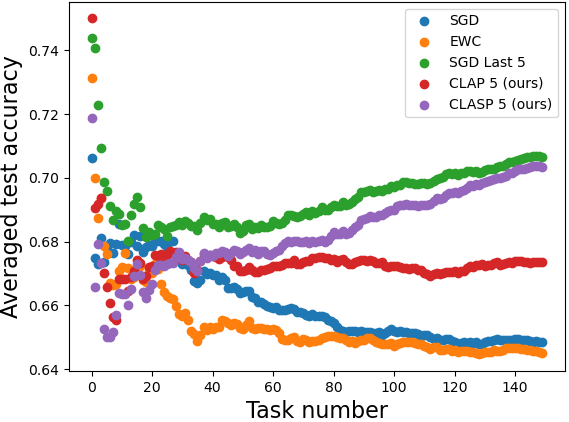
\includegraphics[width=0.26\textwidth]{test_errors_cifar10_static_new}}
\subfigure{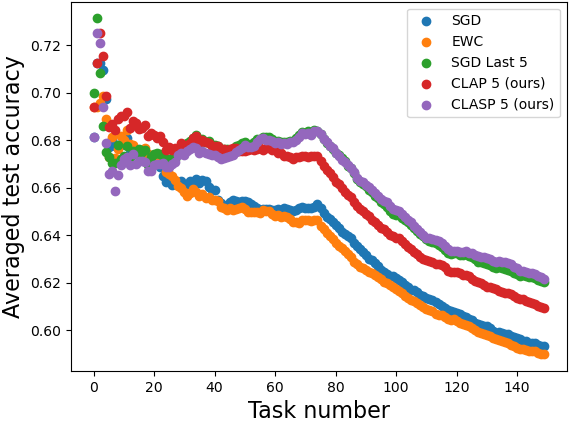
\includegraphics[width=0.26\textwidth]{test_errors_cifar10_shift_new}}
\subfigure{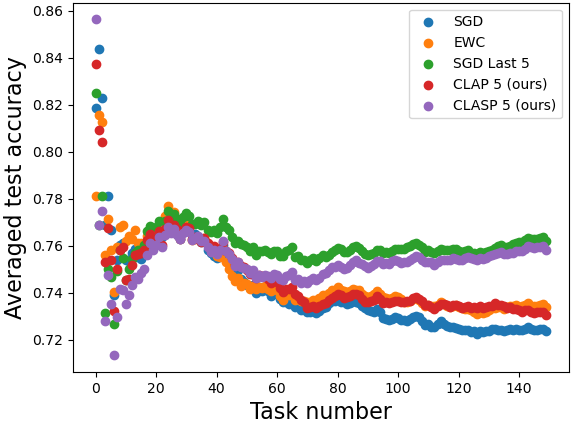
\includegraphics[width=0.26\textwidth]{test_errors_cifar10_random_new}}
\\
\addtocounter{subfigure}{-3}
\subfigure[Domain-incremental\label{cifar-static}]{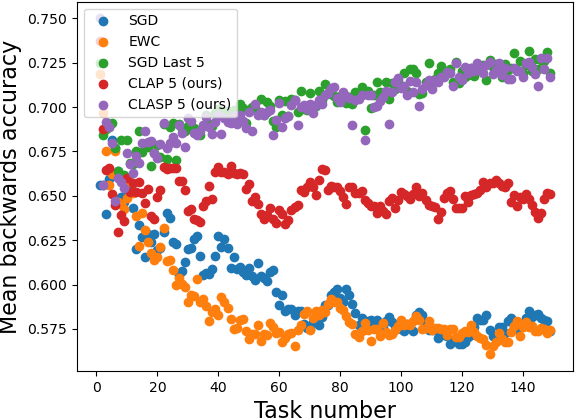
\includegraphics[width=0.26\textwidth]{test_backwards_cifar10_static_new}} 
\subfigure[Shift\label{cifar-shift}]{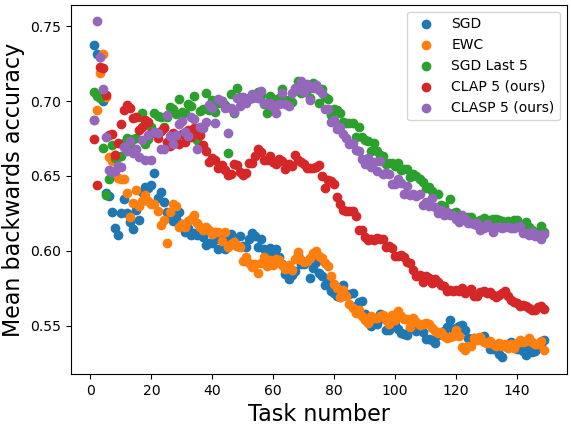
\includegraphics[width=0.26\textwidth]{test_backwards_cifar10_shift_new}} 
\subfigure[Random\label{cifar-random}]{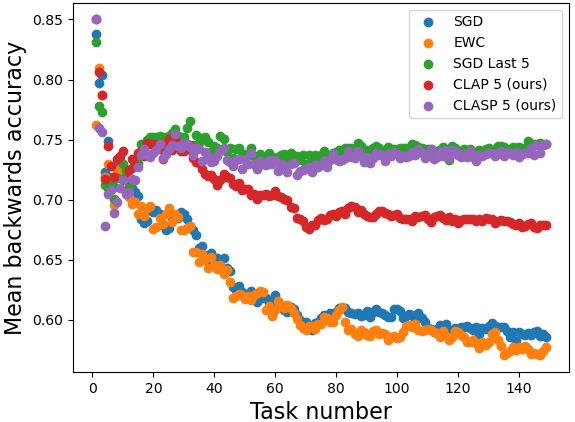
\includegraphics[width=0.26\textwidth]{test_backwards_cifar10_random_new}}

\caption{Metrics over time for the (a) domain-incremental setting (b) domain shift setting (c) random task setting for CIFAR-$10$. Higher is better. Top figures show average test accuracy over time and bottom figures show mean backward accuracy over time.} 
\label{cifar-all}
\end{figure*}

Figure \ref{cifar-static} shows the gradual change in test accuracy and backward transfer.
We can see that after an initial warm-up period, both CLASP and ``last five priors" lead to increasing accuracy as the task distribution is static and previous tasks are highly indicative of future tasks. The more conservative CLAP algorithm displays oscillating average backward transfer, as parameters shift between several modes. The relatively minor improvement of CLASP compared to the last few priors suggests that in most cases $\hat{\mathcal{L}}(\theta_i, S_i)\leq \hat{\mathcal{L}}(\theta_i, S_j)$, and thus they behave similarly overall.
We can also see that the significant improvement in test forgetting coincides with similar improvement in forward transfer. Combined with the reported test accuracy (see Table \ref{cifar-full-table} in Appendix \ref{append:hyperparam}), this suggests that for the domain-incremental setting, backward transfer and forward transfer are strongly linked.%, as one is indicative of the other.

Figure \ref{cifar-shift} details the shifting domain setting. The clear decrease in backward transfer combined with a notable drop in test accuracy immediately after the domain shift may be indicative of issues related to network plasticity and the ``stability-plasticity" dilemma \citep{mirzadeh2020understanding} that is commonly associated with continual learning models based on gradient optimization. Preliminary experiments on longer task horizons suggest that all regularized approaches tend to slowly recover from this issue.

Figure \ref{cifar-random} details the random domain setting. Unsurprisingly, EWC has very poor backward transfer in this setting, as it assumes that there is a shared optimum parameter for all tasks, and this assumption is violated for random tasks. Backward accuracy for other methods seems to plateau at around the $T=80$ mark, though forward transfer does not follow this trend, possibly implying that the representation is rich enough to allow for different parameters to be used for new tasks.

\section{Conclusions} %and future work}

In this work, we derived several upper bounds on the test forgetting (via backward transfer) for both general model classes and for the Gibbs posterior, based on the change of measure approach.
These upper bounds are data-dependent, potentially offering tighter bounds if improved prior models for the task are available, or if tasks are structured such that their loss landscapes are similar. In particular, we focused on oracle bounds for Gibbs posteriors that offered tight bounds on backward transfer if task losses are highly positively correlated, thus making the knowledge accumulation process highly effective for all tasks.

Based on our theoretical bounds, we constructed an algorithm for continual learning with potentially low forgetting that retains and forgets tasks based on the their local loss landscapes. We examined this approach on several simple task constructions as well as a more complex vision task. In our experiments we noted a relation between forward and backward transfer, especially for mostly static settings such as the domain-incremental continual learning problem. As noted by several previous theoretical works and practical examinations (see Introduction), task order and similarity can greatly influence both forgetting and generalization. While this empirical demonstration is not the main focus of our paper, it suggests that weighting schemes based on notions of loss agreement merit further exploration for the domain incremental setting.

%Several interesting directions for future research on general models exist. One relevant extension involves using known literature from Transfer Learning \citep{zhuang2020comprehensive} to allow for bounds where loss landscapes are less similar, as well as better quantifying the effects of this similarity on backward transfer.
%In a somewhat similar vein, it may be useful to derive general bounds that more explicitly consider task order and similarity measures, perhaps using recent advances in PAC-Bayes bounds for Super-martingales \cite{haddouche2023pac}.
%Finally, we can consider more commonly known extensions to PAC-Bayes bounds such as unbounded losses or data-dependent bounds \citep{rivasplata2020pac}.

\clearpage
\bibliographystyle{plainnat}
\bibliography{library}

%%%%%%%%%%%%%%%%%%%%%%%%%%%%%%%%%%%%%%%%%%%%%%%%%%%%%%%%%%%%%%%%%%%%%%%%%%%%%%%
%%%%%%%%%%%%%%%%%%%%%%%%%%%%%%%%%%%%%%%%%%%%%%%%%%%%%%%%%%%%%%%%%%%%%%%%%%%%%%%
% APPENDIX
%%%%%%%%%%%%%%%%%%%%%%%%%%%%%%%%%%%%%%%%%%%%%%%%%%%%%%%%%%%%%%%%%%%%%%%%%%%%%%%
%%%%%%%%%%%%%%%%%%%%%%%%%%%%%%%%%%%%%%%%%%%%%%%%%%%%%%%%%%%%%%%%%%%%%%%%%%%%%%%
\newpage
\appendix
\onecolumn

\section{Appendix - proofs} \label{append:proofs}

% Shui proof actually prove this without the variational lemma, but derivation from the lemma is easy

\begin{lemma} \label{lemma:concentration} \cite{shui2020beyond} Let $\pi$ and $\rho$ be two distributions on a common space $\mathcal{Z}$ such that $\rho$ is absolutely continuous w.\!r.\!t.\! $\pi$. For any $\lambda_t\in \mathbb{R}$ and any measurable function $f:\mathcal{Z}\rightarrow \mathbb{R}$ such that $\mathbb{E}_{z\sim \pi}\left [e^{\lambda_t(f(z)-\mathbb{E}_\pi f(z))} \right ]<\infty$, we have
%
	\begin{equation}
 \begin{split}
	\lambda_t&\left ( \mathbb{E}_{z\sim \rho}\left [f(z) \right ]-\mathbb{E}_{z\sim \pi}\left [f(z) \right ] \right ) \leq 
 D_{\mathrm{KL}}(\rho||\pi)+ \log\mathbb{E}_{z\sim \pi}\left [e^{\lambda_t(f(z)-\mathbb{E}_\pi f(z))} \right ],
 \end{split}
	\end{equation}	
	where $D_{\mathrm{KL}}$ is the KL-divergence and equality is achieved for $f(z)=\mathbb{E}_{z\sim\pi} f(z)+\frac{1}{\lambda_t}\log(\frac{d\rho}{d\pi})$.
\end{lemma}

\begin{theorem} Restatement of Theorem \ref{thm:forget-base2}:
     For any fixed $S_s,S_t,Q_s,Q_{s:t}$, for any $
    \lambda_t>0$,
    \begin{align} 
\begin{split}
\mathcal{L}(Q_{s:t}, \mathcal{D}_s) &\leq \hat{\mathcal{L}}(Q_{s:t}, S_t) + \frac{1}{\lambda_t} D_{\mathrm{KL}}(Q_{s:t}||Q_{s})+\frac{1}{\lambda_t}\log\mathbb{E}_{h\sim Q_{s}}\left [e^{\lambda_t(\mathcal{L}(h,\mathcal{D}_s)-\hat{\mathcal{L}}(h,S_t))} \right ]
\end{split}
\end{align}
\end{theorem}

\begin{proof}
    Starting from Lemma \ref{lemma:concentration}, we can choose $f(z)=\lambda_t(\mathcal{L}(z,\mathcal{D}_s)-\hat{\mathcal{L}}(z,S_t))$, giving us

\begin{align*}
&\lambda_t\mathbb{E}_{h\sim Q_{s:t}}\left [\mathcal{L}(h,\mathcal{D}_s)-\hat{\mathcal{L}}(h,S_t) \right ] - \lambda_t\mathbb{E}_{h\sim Q_{s}}\left [\mathcal{L}(h,\mathcal{D}_s)-\hat{\mathcal{L}}(h,S_t) \right ] \\
&~~\leq D_{\mathrm{KL}}(Q_{s:t}||Q_{s})+\log\mathbb{E}_{h\sim Q_{s}}\left [e^{\lambda_t(\mathcal{L}(h,\mathcal{D}_s)-\hat{\mathcal{L}}(h,S_t))}e^{-\lambda_t(\mathcal{L}(Q_s,\mathcal{D}_s)-\hat{\mathcal{L}}(Q_s,S_t))} \right ]
\end{align*}

Extracting terms that do not depend on $h$ from the expectation, we get

\begin{align} \label{eq:forget-base}
\begin{split}
F(Q_{s:t},\mathcal{D}_s) &\leq \hat{\mathcal{L}}(Q_{s:t}, S_t) - \mathcal{L}(Q_{s}, D_s) + \frac{1}{\lambda_t} D_{\mathrm{KL}}(Q_{s:t}||Q_{s})\\
&+\frac{1}{\lambda_t}\log\mathbb{E}_{h\sim Q_{s}}\left [e^{\lambda_t(\mathcal{L}(h,\mathcal{D}_s)-\hat{\mathcal{L}}(h,S_t))} \right ]
\end{split}
\end{align}

\end{proof}

%%%%%%%%%%%%%%%%%%%%%%%%%%%%%%%%%%%%%%
\begin{lemma} \label{lemma:hoeffding-concentration}
	Let $l:Z\times H\rightarrow[0,K]$ be a measurable function. Let $\pi\in\mathcal{M}(H)$ be a distribution over $H$ that is independent w.r.t. $Z$. Let $S\in Z^m$ be an i.\! i.\! d.\! sample. With probability at least $1-\delta$ over the choice of $S$,
%	
	$$\log \mathbb{E}_{h\sim \pi}\left [e^{t(\frac{1}{m}\sum_i l(z_i,h)-\mathbb{E}_{z}l(z,h))}\right ]\leq \frac{t^2K^2}{8m}+\log{1/ \delta}$$
\end{lemma}

\begin{proof} 
	Using Markov's inequality, we know that 
	$$\textrm{Pr}\left (\mathbb{E}_{h\sim \pi}\left [e^{t(\frac{1}{m}\sum_i l(z_i,h)-\mathbb{E}_{z}l(z,h))}\right ]<\frac{1}{\delta}\mathbb{E}_{S\sim Z^m}\mathbb{E}_{h\sim \pi}\left [e^{t(\frac{1}{m}\sum_i l(z_i,h)-\mathbb{E}_{z}l(z,h))}\right ] \right ) \geq 1-\delta$$
	
	Applying Fubini's theorem (both distributions are independent), we can re-order the expectations
	
	$$\textrm{Pr}\left (\mathbb{E}_{h\sim \pi}\left [e^{t(\frac{1}{m}\sum_i l(z_i,h)-\mathbb{E}_{z}l(z,h))}\right ]<\frac{1}{\delta}\mathbb{E}_{h\sim \pi}\mathbb{E}_{S\sim Z^m}\left [e^{t(\frac{1}{m}\sum_i l(z_i,h)-\mathbb{E}_{z}l(z,h))}\right ] \right ) \geq 1-\delta$$
	
	Since $S$ is drawn i.\! i.\! d.\! and $l$ is bounded, we can apply Hoeffding's lemma to each example, giving us
	
	$$\textrm{Pr}\left (\mathbb{E}_{h\sim \pi}\left [e^{t(\frac{1}{m}\sum_i l(z_i,h)-\mathbb{E}_{z}l(z,h))}\right ]<\frac{1}{\delta}\mathbb{E}_{h\sim \pi}\left [e^{\frac{t^2K^2}{8m}}\right ] \right ) \geq 1-\delta$$
	
	$$\textrm{Pr}\left (\log\mathbb{E}_{h\sim \pi}\left [e^{t(\frac{1}{m}\sum_i l(z_i,h)-\mathbb{E}_{z}l(z,h))}\right ]<\log\frac{1}{\delta}e^{\frac{t^2K^2}{8m}} \right ) \geq 1-\delta$$
	
	and so we have 
	
	$$\textrm{Pr}\left (\log\mathbb{E}_{h\sim \pi}\left [e^{t(\frac{1}{m}\sum_i l(z_i,h)-\mathbb{E}_{z}l(z,h))}\right ]<\log\frac{1}{\delta}+\frac{t^2K^2}{8m} \right ) \geq 1-\delta$$
	
\end{proof}

%%%%%%%%%%%%%%%%%%%%%%%%%%%%%%%%%%%%%%%
%proof for thm:first

\begin{corollary} Restatement of Corollary \ref{thm:first}:
If $\ell\in [0,K]$, for any fixed $S_s,Q_s,Q_{s:t},\lambda_t>0$, with probability at least $1-\delta/2$ over the choice of $S_t$,
\begin{align}
\begin{split}
\mathcal{L}(Q_{s:t}, \mathcal{D}_s) &\leq \hat{\mathcal{L}}(Q_{s:t}, S_t) + \frac{1}{\lambda_t} D_{\mathrm{KL}}(Q_{s:t}||Q_{s})\\
&+\frac{1}{2\lambda_t}\log \mathbb{E}_{h\sim Q_{s}}\left [e^{2\lambda_t(\mathcal{L}(h,\mathcal{D}_s)-\mathcal{L}(h,\mathcal{D}_t))}\right ]+\frac{\lambda_t K^2}{4m_t}+\frac{1}{2\lambda_t}\log(2/\delta)
\end{split}
\end{align}
\end{corollary}

\begin{proof}
    Starting from \eqref{eq:forget-base}, we note that
    $$\log\mathbb{E}_{h\sim Q_{s}}\left [e^{\lambda_t(\mathcal{L}(h,\mathcal{D}_s)-\hat{\mathcal{L}}(h,S_t))} \right ] = \log\mathbb{E}_{h\sim Q_{s}}\left [e^{\lambda_t(\mathcal{L}(h,\mathcal{D}_s)-\mathcal{L}(h,\mathcal{D}_t)+\mathcal{L}(h,\mathcal{D}_t)-\hat{\mathcal{L}}(h,S_t))} \right ].$$

    This gives us 
\begin{align*}
\log\mathbb{E}_{h\sim Q_{s}}\left [e^{\lambda_t(\mathcal{L}(h,\mathcal{D}_s)-\hat{\mathcal{L}}(h,S_t))} \right] &= \log\mathbb{E}_{h\sim Q_{s}}\left [e^{\lambda_t(\mathcal{L}(h,\mathcal{D}_s)-\mathcal{L}(h,\mathcal{D}_t))}e^{\lambda_t(\mathcal{L}(h,\mathcal{D}_t)-\hat{\mathcal{L}}(h,S_t))} \right ]\\
&\triangleq \log\mathbb{E}_{Q_{s}}\left [e^{\lambda_t\Delta\mathcal{L}(h,\mathcal{D}_s, \mathcal{D}_t)}e^{\lambda_t\Delta\hat{\mathcal{L}}(h,\mathcal{D}_t, S_t)} \right ].
\end{align*}

Using the Cauchy-Schwartz inequality $$\mathbb{E}_{X}\left [f_1(X)f_2(X)\right ]^2\leq \mathbb{E}_{X}\left [f_1(X)^2\right ]\mathbb{E}_{X}\left [f_2(X)^2\right ],$$
as well as the fact that both exponent terms are non-negative, we have

\begin{align} \label{eq:cs-diff}
\begin{split}
\log\mathbb{E}_{Q_{s}}\left [e^{\lambda_t\Delta\mathcal{L}(h,\mathcal{D}_s, \mathcal{D}_t)}e^{\lambda_t\Delta\hat{\mathcal{L}}(h,\mathcal{D}_t, S_t)} \right ]\leq \frac{1}{2}\log\mathbb{E}_{Q_{s}}\left [e^{2\lambda_t\Delta\mathcal{L}(h,\mathcal{D}_s, \mathcal{D}_t)}\right ]\mathbb{E}_{Q_{s}}\left [e^{2\lambda_t\Delta\hat{\mathcal{L}}(h,\mathcal{D}_t, S_t)} \right ].
\end{split}
\end{align}

If $\ell\in [0,K]$, we can use Lemma \ref{lemma:hoeffding-concentration} and \eqref{eq:cs-diff} and get with probability at least $1-\delta/2$ over the choice of $S_t$

$$\log\mathbb{E}_{h\sim Q_{s}}\left [e^{\lambda_t(\mathcal{L}(h,\mathcal{D}_s)-\hat{\mathcal{L}}(h,S_t))} \right ]\leq \frac{1}{2}\log\mathbb{E}_{Q_{s}}\left [e^{2\lambda_t\Delta\mathcal{L}(h,\mathcal{D}_s, \mathcal{D}_t)}\right ]+\frac{\lambda_t^2K^2}{4m_t}+\log(2/\delta)$$

\end{proof}

%%%%%%%%%%%%%%%%%%%%%%%%%%%%%%%%%%%%%%%%%%%
% proof for gibbs general

\begin{corollary} Restatement of Corollary \ref{thm:gibbs-general}:
For any $\lambda_t>0$, if $$Q_s(h)=\frac{P(h)e^{-2\lambda_t\hat{\mathcal{L}}(h,S_s)}}{\mathbb{E}_{h\sim P}\left [e^{-2\lambda_t\hat{\mathcal{L}}(h,S_s)} \right ]}$$ and the loss is bounded $\ell\in[0,K]$, 
we have with probability at least $1-\delta/2$ over the choice of $S_s,S_t$, for any $Q_{s:t}$, 
%
\begin{align}
\begin{split}
\mathcal{L}(Q_{s:t}, \mathcal{D}_s) &\leq \hat{\mathcal{L}}(Q_{s:t}, S_t) + \frac{1}{\lambda_t} D_{\mathrm{KL}}(Q_{s:t}||Q_{s})\\
&+\frac{\lambda_t K^2}{4m_s}+\frac{\lambda_t K^2}{4m_t}+\frac{1}{\lambda_t}\log(2/\delta)+ \hat{\mathcal{L}}(P, S_s)
\end{split}
\end{align}
\end{corollary}

\begin{proof}
    Starting from Corollary \ref{thm:first}, we note that
    $$\frac{1}{2\lambda_t}\log \mathbb{E}_{h\sim Q_{s}}\left [e^{2\lambda_t(\mathcal{L}(h,\mathcal{D}_s)-\mathcal{L}(h,\mathcal{D}_t))}\right ]$$
    $$=\frac{1}{2\lambda_t}\log \int \frac{1}{\mathbb{E}_{h\sim P}\left [e^{-2\lambda_t\hat{\mathcal{L}}(h,S_s)} \right ]}P(h)e^{2\lambda_t(\mathcal{L}(h,\mathcal{D}_s)-\hat{\mathcal{L}}(h,S_s)-\mathcal{L}(h,\mathcal{D}_t))}dh$$
    $$=\frac{1}{2\lambda_t}\log \int \frac{\mathbb{E}_{h\sim P} e^{-2\lambda_t\mathcal{L}(h,\mathcal{D}_t)}}{\mathbb{E}_{h\sim P} e^{-2\lambda_t\hat{\mathcal{L}}(h,S_s)}  }\frac{P(h)e^{-2\lambda_t\mathcal{L}(h,\mathcal{D}_t)}}{\mathbb{E}_{h\sim P} e^{-2\lambda_t\mathcal{L}(h,\mathcal{D}_t)}}e^{2\lambda_t(\mathcal{L}(h,\mathcal{D}_s)-\hat{\mathcal{L}}(h,S_s))}dh$$
    $$=\frac{1}{2\lambda_t}\log\frac{\mathbb{E}_{h\sim P} e^{-2\lambda_t\mathcal{L}(h,\mathcal{D}_t)}}{\mathbb{E}_{h\sim P} e^{-2\lambda_t\hat{\mathcal{L}}(h,S_s)}  }+\frac{1}{2\lambda_t}\log\mathbb{E}_{h\sim Q^{*}_t}\left [e^{2\lambda_t(\mathcal{L}(h,\mathcal{D}_s)-\hat{\mathcal{L}}(h,S_s))}\right ]$$

    Using Lemma \ref{lemma:hoeffding-concentration} again gives us with probability at least $1-\delta/2$ over the choice of $S_s$

$$\frac{1}{2\lambda_t}\log \mathbb{E}_{h\sim Q^{*}_t}\left [e^{2\lambda_t(\mathcal{L}(h,\mathcal{D}_s)-\mathcal{L}(h,\mathcal{D}_t))}\right ] \leq \frac{\lambda_t K^2}{4m_s}+\frac{1}{2\lambda_t}\log(2/\delta)$$

Putting it all together with a union bound, if $Q_s(h)=\frac{P(h)e^{-2\lambda_t\hat{\mathcal{L}}(h,S_s)}}{\mathbb{E}_{h\sim P}\left [e^{-2\lambda_t\hat{\mathcal{L}}(h,S_s)} \right ]}$ and the loss is bounded $\ell\in[0,K]$, we have with probability at least $1-\delta/2$ over the choice of $S_s,S_t$,

\begin{align}
\begin{split}
\mathcal{L}(Q_{s:t}, \mathcal{D}_s) &\leq \hat{\mathcal{L}}(Q_{s:t}, S_t) + \frac{1}{\lambda_t} D_{\mathrm{KL}}(Q_{s:t}||Q_{s})
+\frac{\lambda_t K^2}{4m_s}+\frac{\lambda_t K^2}{4m_t}+\\&\frac{1}{\lambda_t}\log(2/\delta)+\frac{1}{2\lambda_t}\log\frac{\mathbb{E}_{h\sim P} e^{-2\lambda_t\mathcal{L}(h,\mathcal{D}_t)}}{\mathbb{E}_{h\sim P} e^{-2\lambda_t\hat{\mathcal{L}}(h,S_s)}  }
\end{split}
\end{align}

We can further simplify this expression 

\begin{align*}
\begin{split}
\mathcal{L}(Q_{s:t}, \mathcal{D}_s) &\leq \hat{\mathcal{L}}(Q_{s:t}, S_t)+ \frac{1}{\lambda_t} D_{\mathrm{KL}}(Q_{s:t}||Q_{s})
+\frac{\lambda_t K^2}{4m_s}+\frac{\lambda_t K^2}{4m_t}+\frac{1}{\lambda_t}\log(2/\delta)\\&+\frac{1}{2\lambda_t}\log\mathbb{E}_{h\sim P} e^{-2\lambda_t\mathcal{L}(h,\mathcal{D}_t)}-\frac{1}{2\lambda_t}\log\mathbb{E}_{h\sim P} e^{-2\lambda_t\hat{\mathcal{L}}(h,S_s)}   \\
& \leq \hat{\mathcal{L}}(Q_{s:t}, S_t)+ \frac{1}{\lambda_t} D_{\mathrm{KL}}(Q_{s:t}||Q_{s})
+\frac{\lambda_t K^2}{4m_s}+\frac{\lambda_t K^2}{4m_t}+\frac{1}{\lambda_t}\log(2/\delta)\\&+0+\frac{1}{2\lambda_t}\mathbb{E}_{h\sim P} 2\lambda_t\hat{\mathcal{L}}(h,S_s) \\
& \leq \hat{\mathcal{L}}(Q_{s:t}, S_t) + \frac{1}{\lambda_t} D_{\mathrm{KL}}(Q_{s:t}||Q_{s})
+\frac{\lambda_t K^2}{4m_s}+\frac{\lambda_t K^2}{4m_t}+\frac{1}{\lambda_t}\log(2/\delta)+ \hat{\mathcal{L}}(P, S_s)
\end{split}
\end{align*}

\end{proof}

%%%%%%%%%%%%%%%%%%%%%%%%%%%%%%%%%%%%%%%%%%%%%%

%proof for oracle:base

\begin{theorem} Restatement of Theorem \ref{thm:oracle-base}:
For any $Q_s, S_s, \lambda_t>0$, if $\ell\in [0,K]$, 
\begin{equation} 
\begin{split}
\mathbb{E}_{S_t\sim \mathcal{D}_t}&\mathcal{L}( \hat{Q}^{\lambda_t}_{s:t},\mathcal{D}_s)\leq\inf_{Q_{s:t}}\left \{ \mathcal{L}(Q_{s:t},\mathcal{D}_t) + \frac{1}{\lambda_t}D_{\mathrm{KL}}(Q_{s:t}||Q_{s}) \right \} \\
&+\frac{\lambda_t K^2}{8m_t}+\frac{1}{\lambda_t}\log\mathbb{E}_{h\sim Q_s}\left [e^{\lambda_t(\mathcal{L}(h,\mathcal{D}_s)-\mathcal{L}(h,\mathcal{D}_t))} \right ]
\end{split}
\end{equation}
\end{theorem}

\begin{proof}
Starting from Lemma \ref{lemma:concentration}, we know that 

$$\mathbb{E}_{z\sim \rho}\left [f(z) \right ]\leq \mathbb{E}_{z\sim \pi}\left [f(z) \right ]+ \frac{1}{\lambda_t}D_{\mathrm{KL}}(\rho||\pi)+ \frac{1}{\lambda_t}\log\mathbb{E}_{z\sim \pi}\left [e^{\lambda_t(f(z)-\mathbb{E}_\pi f(z))} \right ]$$

In particular, for $\hat{\rho}_\lambda(z)\propto \pi(z) e^{-\lambda_t f(z) }$, this is an equality (from \citeauthor{donsker1975large}'s [\citeyear{donsker1975large}] variational lemma).
From this, we know that

\begin{equation}
\mathbb{E}_{z\sim \hat{\rho}_\lambda}\left [f(z) \right ]= \mathbb{E}_{z\sim \pi}\left [f(z) \right ]+ \frac{1}{\lambda_t}D_{\mathrm{KL}}(\hat{\rho}_\lambda||\pi)+ \frac{1}{\lambda_t}\log\mathbb{E}_{z\sim \pi}\left [e^{\lambda_t(f(z)-\mathbb{E}_\pi f(z))} \right ]
\end{equation}

If we pick $f(z)=\mathcal{L}(z,\mathcal{D}_s)-\hat{\mathcal{L}}(z,S_t)$ as before, we get

\begin{equation*} 
\begin{split}
\mathbb{E}_{z\sim \hat{\rho}_\lambda}\left [\mathcal{L}(z,\mathcal{D}_s) \right ]&= \mathbb{E}_{z\sim \pi}\left [f(z) \right ]+\mathbb{E}_{z\sim \hat{\rho}_\lambda}\left [\hat{\mathcal{L}}(z,S_t) \right ]+ \frac{1}{\lambda_t}D_{\mathrm{KL}}(\hat{\rho}_\lambda||\pi)\\&+ \frac{1}{\lambda_t}\log\mathbb{E}_{z\sim \pi}\left [e^{\lambda_t(f(z)-\mathbb{E}_\pi f(z))} \right ]
\end{split}
\end{equation*}

And as such,
$$F( \hat{\rho}_\lambda,\mathcal{D}_s)\leq \inf_{\rho}\left \{ \hat{\mathcal{L}}(\rho,S_t) + \frac{1}{\lambda_t}D_{\mathrm{KL}}(\rho||\pi)  \right \}-\mathcal{L}(\pi,D_s)+\frac{1}{\lambda_t}\log\mathbb{E}_{z\sim \pi}\left [e^{\lambda_t(\mathcal{L}(z,\mathcal{D}_s)-\hat{\mathcal{L}}(z,S_t))} \right ],$$

or using our previous terminology with $\hat{Q}^{\lambda_t}_{s:t}(h)\propto Q_s(h)e^{-\lambda_t\hat{\mathcal{L}}(h,S_t)}$, 

$$\mathcal{L}( \hat{Q}^{\lambda_t}_{s:t},\mathcal{D}_s)\leq \inf_{Q_{s:t}}\left \{ \hat{\mathcal{L}}(Q_{s:t},S_t) + \frac{1}{\lambda_t}D_{\mathrm{KL}}(Q_{s:t}||Q_{s}) \right \}+\frac{1}{\lambda_t}\log\mathbb{E}_{h\sim Q_s}\left [e^{\lambda_t(\mathcal{L}(h,\mathcal{D}_s)-\hat{\mathcal{L}}(h,S_t))} \right ]$$

If we take an expectation on $S_t$, we get

\begin{equation*} 
\begin{split}
\mathbb{E}_{S_t\sim \mathcal{D}_t}\mathcal{L}( \hat{Q}^{\lambda_t}_{s:t},\mathcal{D}_s)&\leq \mathbb{E}_{S_t\sim \mathcal{D}_t}\inf_{Q_{s:t}}\left \{ \hat{\mathcal{L}}(Q_{s:t},S_t) + \frac{1}{\lambda_t}D_{\mathrm{KL}}(Q_{s:t}||Q_{s}) \right \}\\&+\frac{1}{\lambda_t}\mathbb{E}_{S_t\sim \mathcal{D}_t}\log\mathbb{E}_{h\sim Q_s}\left [e^{\lambda_t(\mathcal{L}(h,\mathcal{D}_s)-\hat{\mathcal{L}}(h,S_t))} \right ]
\end{split}
\end{equation*}


This gives us the following oracle inequality (in expectation):

\begin{equation*} 
\begin{split}
\mathbb{E}_{S_t\sim \mathcal{D}_t}\mathcal{L}( \hat{Q}^{\lambda_t}_{s:t},\mathcal{D}_s)&\leq \inf_{Q_{s:t}}\left \{ \mathcal{L}(Q_{s:t},\mathcal{D}_t) + \frac{1}{\lambda_t}D_{\mathrm{KL}}(Q_{s:t}||Q_{s}) \right \}\\&+\frac{1}{\lambda_t}\log\mathbb{E}_{h\sim Q_s}\mathbb{E}_{S_t\sim \mathcal{D}_t}\left [e^{\lambda_t(\mathcal{L}(h,\mathcal{D}_s)-\hat{\mathcal{L}}(h,S_t))} \right ]
\end{split}
\end{equation*}

We have

$$\frac{1}{\lambda_t}\log\mathbb{E}_{h\sim Q_s}\mathbb{E}_{S_t\sim \mathcal{D}_t}\left [e^{\lambda_t(\mathcal{L}(h,\mathcal{D}_s)-\hat{\mathcal{L}}(h,S_t))} \right ]$$
$$=\frac{1}{\lambda_t}\log\mathbb{E}_{h\sim Q_s}\mathbb{E}_{S_t\sim \mathcal{D}_t}\left [e^{\lambda_t(\mathcal{L}(h,\mathcal{D}_s)-\mathcal{L}(h,\mathcal{D}_t))}e^{\lambda_t(\mathcal{L}(h,\mathcal{D}_t)-\hat{\mathcal{L}}(h,S_t))} \right ]$$

$$=\frac{1}{\lambda_t}\log\mathbb{E}_{h\sim Q_s}\left [e^{\lambda_t(\mathcal{L}(h,\mathcal{D}_s)-\mathcal{L}(h,\mathcal{D}_t))}\mathbb{E}_{S_t\sim \mathcal{D}_t}e^{\lambda_t(\mathcal{L}(h,\mathcal{D}_t)-\hat{\mathcal{L}}(h,S_t))} \right ]$$

Using Hoeffding's lemma, we get

$$\frac{1}{\lambda_t}\log\mathbb{E}_{h\sim Q_s}\mathbb{E}_{S_t\sim \mathcal{D}_t}\left [e^{\lambda_t(\mathcal{L}(h,\mathcal{D}_s)-\hat{\mathcal{L}}(h,S_t))} \right ] \leq \frac{\lambda_t K^2}{8m_t}+\frac{1}{\lambda_t}\log\mathbb{E}_{h\sim Q_s}\left [e^{\lambda_t(\mathcal{L}(h,\mathcal{D}_s)-\mathcal{L}(h,\mathcal{D}_t))} \right ]$$

\end{proof}


%%%%%%%%%%%%%%%%%%%%%%%%%%%%%%%%%%%%%%%%%%%%%%
%bound for similr tsks oorcle bound

Proof of accompanying Corollary:
\begin{proof}
From our assumption $0\leq \mathrm{Dis}(Q_s,\mathcal{D}_s, \mathcal{D}_t, \lambda_t ) \leq \epsilon_{s,t}$ we also have $0\leq |\mathcal{L}(Q_s,\mathcal{D}_s)-\mathcal{L}(Q_s,\mathcal{D}_t)|
\leq \epsilon_{s,t}$

Looking at the negative transfer, we see
\begin{equation*}
\mathbb{E}_{S_s\sim \mathcal{D}_s}\mathbb{E}_{S_t\sim \mathcal{D}_t}F(\hat{Q}^{\lambda_t}_{s:t},\mathcal{D}_t)\leq \mathbb{E}_{S_s\sim \mathcal{D}_s}\left [\mathcal{L}(Q_{s},\mathcal{D}_t)-\mathcal{L}(Q_{s},\mathcal{D}_s)\right ]+\frac{\lambda_t K^2}{8m_t} + \epsilon_{s,t}
\end{equation*}

and similarly from our assumption, we have
\begin{equation*}
\mathbb{E}_{S_s\sim \mathcal{D}_s}\mathbb{E}_{S_t\sim \mathcal{D}_t}F(\hat{Q}^{\lambda_t}_{s:t},\mathcal{D}_t)\leq \frac{\lambda_t K^2}{8m_t} + 2\epsilon_{s,t}
\end{equation*}

\end{proof}

%%%%%%%%%%%%%%%%%%%%%%%%%%%%%%%%%%%%%%%%%%%%
%oracle bounds discrepency

\begin{corollary} Restatement of Corollary \ref{thm:oracle-logsum}:
If $\ell\in[0,K]$, for any given $S_s\sim \mathcal{D}_s, Q_s, \lambda_t>0$, 
%
\begin{equation} 
\begin{split}
\mathbb{E}_{S_t\sim \mathcal{D}_t}&\mathcal{L}( \hat{Q}^{\lambda_t}_{s:t},\mathcal{D}_s)\leq \frac{\lambda_t K^2}{8m_t}+\frac{\mathbb{E}_{h\sim Q_s}\left [e^{\lambda_t(\mathcal{L}(h,\mathcal{D}_s)-\mathcal{L}(h,\mathcal{D}_t))}\mathcal{L}(h,\mathcal{D}_s) \right ]}{\mathbb{E}_{h\sim Q_s}\left [e^{\lambda_t(\mathcal{L}(h,\mathcal{D}_s)-\mathcal{L}(h,\mathcal{D}_t))}\right ]}
\end{split}
\end{equation}
\end{corollary}

\begin{proof}
We can derive such a bound using \eqref{eq:oracle-base} by setting the optimal posterior:

\begin{equation*} 
\begin{split}
\mathbb{E}_{S_t\sim \mathcal{D}_t}\mathcal{L}( \hat{Q}^{\lambda_t}_{s:t},\mathcal{D}_s)&\leq -\frac{1}{\lambda_t}\log \mathbb{E}_{h\sim Q_s}\left [e^{-\lambda_t\mathcal{L}(h,\mathcal{D}_t)}\right ]\\&+\frac{\lambda_t K^2}{8m_t}+\frac{1}{\lambda_t}\log\mathbb{E}_{h\sim Q_s}\left [e^{\lambda_t(\mathcal{L}(h,\mathcal{D}_s)-\mathcal{L}(h,\mathcal{D}_t))} \right ]
\end{split}
\end{equation*}

This is the same as writing

$$
\mathbb{E}_{S_t\sim \mathcal{D}_t}\mathcal{L}( \hat{Q}^{\lambda_t}_{s:t},\mathcal{D}_s)\leq \frac{\lambda_t K^2}{8m_t}+\frac{1}{\lambda_t}\log\frac{\mathbb{E}_{h\sim Q_s}\left [e^{\lambda_t(\mathcal{L}(h,\mathcal{D}_s)-\mathcal{L}(h,\mathcal{D}_t))} \right ]}{\mathbb{E}_{h\sim Q_s}\left [e^{-\lambda_t\mathcal{L}(h,\mathcal{D}_t)}\right ]}
$$

Since $e^k\geq 0$ for all $k\in \mathbb{R}$, we can apply the log-sum inequality:

$$
\mathbb{E}_{S_t\sim \mathcal{D}_t}\mathcal{L}( \hat{Q}^{\lambda_t}_{s:t},\mathcal{D}_s)\leq \frac{\lambda_t K^2}{8m_t}+\frac{1}{\lambda_t}\frac{\mathbb{E}_{h\sim Q_s}\left [e^{\lambda_t(\mathcal{L}(h,\mathcal{D}_s)-\mathcal{L}(h,\mathcal{D}_t))}\log\frac{e^{\lambda_t(\mathcal{L}(h,\mathcal{D}_s)-\mathcal{L}(h,\mathcal{D}_t))}}{e^{\lambda_t(-\mathcal{L}(h,\mathcal{D}_t))}} \right ]}{\mathbb{E}_{h\sim Q_s}\left [e^{\lambda_t(\mathcal{L}(h,\mathcal{D}_s)-\mathcal{L}(h,\mathcal{D}_t))}\right ]}
$$
\end{proof}

%%%%%%%%%%%%%

\begin{corollary} %Restatement of %Corollary %\ref{thm:oracle-final}:
\label{corollary:appendix}
Appendix-only Corollary:
If $\ell\in[0,K]$, for any given $Q_s, \lambda_t>0, S_s\sim \mathcal{D}_s$,  
%
\begin{equation} \label{eq:oracle-final}
\begin{split}
\mathbb{E}_{S_t\sim \mathcal{D}_t}\mathcal{L}( \hat{Q}^{\lambda_t}_{s:t},&\mathcal{D}_s)\leq \frac{\lambda_t K^2}{8m_t}\\&+\frac{\sqrt{\mathbb{E}_{Q_s}\left [e^{2\lambda_t(\mathcal{L}(h,\mathcal{D}_s)-\mathcal{L}(h,\mathcal{D}_t))}\right ]}}{\mathbb{E}_{Q_s}\left [e^{\lambda_t(\mathcal{L}(h,\mathcal{D}_s)-\mathcal{L}(h,\mathcal{D}_t))}\right ]}\cdot \left (\sqrt{\mathrm{Var}_{Q_s}(\mathcal{L}(h,\mathcal{D}_s))}+\mathcal{L}(Q_s,\mathcal{D}_s)\right )
\end{split}
\end{equation}
\end{corollary}

\begin{proof}
Starting from \eqref{eq:oracle-logsum}, we can apply the Cauchy-Schwartz theorem on the expectation and get

$$
\mathbb{E}_{S_t\sim \mathcal{D}_t}\mathcal{L}( \hat{Q}^{\lambda_t}_{s:t},\mathcal{D}_s)\leq \frac{\lambda_t K^2}{8m_t}+\frac{\sqrt{\mathbb{E}_{Q_s}\left [e^{2\lambda_t(\mathcal{L}(h,\mathcal{D}_s)-\mathcal{L}(h,\mathcal{D}_t))}\right ]\mathbb{E}_{Q_s}\left [\mathcal{L}(h,\mathcal{D}_s)^2 \right ]}}{\mathbb{E}_{Q_s}\left [e^{\lambda_t(\mathcal{L}(h,\mathcal{D}_s)-\mathcal{L}(h,\mathcal{D}_t))}\right ]};
$$

\begin{equation} \label{eq:oracle-CS-opt}
=\frac{\lambda_t K^2}{8m_t}+\frac{\sqrt{\mathbb{E}_{Q_s}\left [e^{2\lambda_t(\mathcal{L}(h,\mathcal{D}_s)-\mathcal{L}(h,\mathcal{D}_t))}\right ]}}{\mathbb{E}_{Q_s}\left [e^{\lambda_t(\mathcal{L}(h,\mathcal{D}_s)-\mathcal{L}(h,\mathcal{D}_t))}\right ]}\sqrt{\mathbb{E}_{Q_s}\left [\mathcal{L}(h,\mathcal{D}_s)^2 \right ]}
\end{equation}

And using the definition of variance and the triangle inequality (since both terms are non-negative), we get \eqref{eq:oracle-final}.

\end{proof}


%%%%%%%%%%%%%%%%%%%%%%%%%%%%%%%%%%%%%%%%%%%%%%%%%%%%%%%%

\begin{theorem} Restatement of Theorem \ref{thm:forgetting-extended}:
For any $\lambda_T>0$, assuming all $Q_{1:j}$ are empirical Gibbs posteriors, $\ell\in[0,K]$, and that
 $\mathrm{cov}_{P}(e^{-\lambda_T\hat{\mathcal{L}}(h,S_i)}, e^{-\sum_{j=1,j\neq i}^{T}\lambda_j\hat{\mathcal{L}}(h,S_j)})\geq 0$,
for any sample of training sets $S_{j}\sim \mathcal{D}_j$,
%
\begin{align} 
\begin{split}
\forall i\in[1,T-1]:
\mathbb{E}_{S_i}\mathcal{L}(\hat{Q}^{\lambda_T}_{1:T}, \mathcal{D}_i) &\leq \frac{\lambda_T K^2}{8m_i}+\mathcal{L}(P,\mathcal{D}_i)
\end{split}
\end{align}
\end{theorem}

\begin{proof}
    Starting from \eqref{eq:forget-base-T}, suppose we assume that for each task we apply an empirical Gibbs learner, meaning $$\forall i\in[2,T], \hat{Q}^{\lambda_i}_{1:i}(h)\propto \hat{Q}^{\lambda_{i-1}}_{1:i-1}(h)e^{-\lambda_i\hat{\mathcal{L}}(h,S_i)}$$ 
where $\hat{Q}^{\lambda_1}_{1:1}(h)\propto P(h)e^{-\lambda_1\hat{\mathcal{L}}(h,S_1)}$.

We can provide bounds on the forgetting of $\hat{Q}^{\lambda_T}_{1:T}$ by setting the posterior $Q_{1:T}$ and the prior $Q_{1:T-1}$ as Gibbs posteriors:


\begin{align*} 
\begin{split}
\forall i\in[1,T-1]:
\mathcal{L}(\hat{Q}^{\lambda_T}_{1:T}, \mathcal{D}_i) &\leq \frac{1}{\lambda_T}\log\frac{\mathbb{E}_{h\sim \hat{Q}^{\lambda_{T-1}}_{1:T-1}}\left [e^{\lambda_T(\mathcal{L}(h,\mathcal{D}_i)-\hat{\mathcal{L}}(h,S_T))} \right ]}{\mathbb{E}_{h\sim \hat{Q}^{\lambda_{T-1}}_{1:T-1}}\left [e^{-\lambda_T\hat{\mathcal{L}}(h,S_T)} \right ]}
\end{split}
\end{align*}

We can unravel the expectations and arrive at:

\begin{align*} 
\begin{split}
\forall i\in[1,T-1]:
\mathcal{L}(\hat{Q}^{\lambda_T}_{1:T}, \mathcal{D}_i) &\leq \frac{1}{\lambda_T}\log\frac{\mathbb{E}_{h\sim P}\left [e^{\lambda_T\mathcal{L}(h,\mathcal{D}_i)-\sum_{j=1}^{T}\lambda_j\hat{\mathcal{L}}(h,S_j)} \right ]}{\mathbb{E}_{h\sim P}\left [e^{-\sum_{j=1}^{T}\lambda_j\hat{\mathcal{L}}(h,S_j)} \right ]}
\end{split}
\end{align*}

Taking an expectation over $S_i$,

\begin{align*} 
\begin{split}
\forall i\in[1,T-1]:
\mathbb{E}_{S_i}\mathcal{L}(\hat{Q}^{\lambda_T}_{1:T}, \mathcal{D}_i) &\leq \frac{1}{\lambda_T}\mathbb{E}_{S_i}\log\frac{\mathbb{E}_{h\sim P}\left [e^{\lambda_T\mathcal{L}(h,\mathcal{D}_i)-\sum_{j=1}^{T}\lambda_j\hat{\mathcal{L}}(h,S_j)} \right ]}{\mathbb{E}_{h\sim P}\left [e^{-\sum_{j=1}^{T}\lambda_j\hat{\mathcal{L}}(h,S_j)} \right ]}
\end{split}
\end{align*}

Applying Jensen's inequality:

\begin{align*} 
\begin{split}
\forall i\in[1,T-1]:
&\mathbb{E}_{S_i}\mathcal{L}(\hat{Q}^{\lambda_T}_{1:T}, \mathcal{D}_i) \\&\leq \frac{1}{\lambda_T}\mathbb{E}_{S_i}\log\frac{\mathbb{E}_{h\sim P}\left [\mathbb{E}_{S_i}\left [e^{\lambda_T\mathcal{L}(h,\mathcal{D}_i)-\lambda_i\hat{\mathcal{L}}(h,S_i)} \right ]e^{-\sum_{j=1,j\neq i}^{T}\lambda_j\hat{\mathcal{L}}(h,S_j)} \right ]}{\mathbb{E}_{h\sim P}\left [e^{-\sum_{j=1}^{T}\lambda_j\hat{\mathcal{L}}(h,S_j)} \right ]}
\end{split}
\end{align*}

If $\lambda_i=\lambda_T$, we can apply Hoeffding's lemma:

\begin{align*} 
\begin{split}
\forall i\in[1,T-1]:
\mathbb{E}_{S_i}\mathcal{L}(\hat{Q}^{\lambda_T}_{1:T}, \mathcal{D}_i) &\leq \frac{\lambda_T K^2}{8m_i}+\frac{1}{\lambda_T}\mathbb{E}_{S_i}\log\frac{\mathbb{E}_{h\sim P}\left [e^{-\sum_{j=1,j\neq i}^{T}\lambda_j\hat{\mathcal{L}}(h,S_j)} \right ]}{\mathbb{E}_{h\sim P}\left [e^{-\sum_{j=1}^{T}\lambda_j\hat{\mathcal{L}}(h,S_j)} \right ]}
\end{split}
\end{align*}

As in the paper, we mark 
$$\mathrm{cov}_{P}(i, [T])\triangleq\mathrm{cov}_{P}(e^{-\lambda_T\hat{\mathcal{L}}(h,S_i)}, e^{-\sum_{j=1,j\neq i}^{T}\lambda_j\hat{\mathcal{L}}(h,S_j)}).$$

From the definition of covariance, we can decompose the denominator:

\begin{align} \label{eq-oracle-forget-extend}
\begin{split}
&\forall i\in[1,T-1]:
\mathbb{E}_{S_i}\mathcal{L}(\hat{Q}^{\lambda_T}_{1:T}, \mathcal{D}_i) \leq \frac{\lambda_T K^2}{8m_i}\\&+\frac{1}{\lambda_T}\mathbb{E}_{S_i}\log\frac{\mathbb{E}_{h\sim P}\left [e^{-\sum_{j=1,j\neq i}^{T}\lambda_j\hat{\mathcal{L}}(h,S_j)} \right ]}{\mathbb{E}_{h\sim P}\left [e^{-\sum_{j=1,j\neq i}^{T}\lambda_j\hat{\mathcal{L}}(h,S_j)} \right ]\mathbb{E}_{h\sim P}\left [e^{-\lambda_T\hat{\mathcal{L}}(h,S_i)} \right ]+\mathrm{cov}_{P}(i, [T])}
\end{split}
\end{align}

And if this covariance is non-negative, we can set it at $0$ and still retain a valid upper bound, giving us the forgetting bound via Jensen's inequality.

Similarly for forward transfer, we get 

\begin{align} \label{eq-oracle-forward-extend}
\begin{split}
&\mathbb{E}_{S_T}\mathcal{L}(\hat{Q}^{\lambda_T}_{1:T}, \mathcal{D}_T) \leq \frac{\lambda_T K^2}{8m_T}\\&+
\frac{1}{\lambda_T}\mathbb{E}_{S_T}\log\frac{\mathbb{E}_{h\sim P}\left [e^{-\sum_{j=1}^{T-1}\lambda_j\hat{\mathcal{L}}(h,S_j)} \right ]}{\mathbb{E}_{h\sim P}\left [e^{-\sum_{j=1}^{T-1}\lambda_j\hat{\mathcal{L}}(h,S_j)} \right ]\mathbb{E}_{h\sim P}\left [e^{-\lambda_T\hat{\mathcal{L}}(h,S_T)} \right ]+\mathrm{cov}_{P}(T, [T])}
\end{split}
\end{align}

and apply $\mathrm{cov}_{P}(T, [T])\geq 0$ and Jensen's inequality to get the bound for generalization.

\end{proof}

%%%%%%%%%%%%%%%%%%%%%%%%%%%%%%%%%%%%%%%%%%%%%%%

\begin{corollary} \label{thm:oracle-T-highcov}:
    Appendix-only Corollary: Under the same conditions as Theorem \ref{thm:forgetting-extended}, if we additionally have
%
\begin{align*} 
\begin{split}
\mathrm{cov}_{P}(e^{-\lambda_T\hat{\mathcal{L}}(h,S_i)}, e^{-\sum_{j=1,j\neq i}^{T}\lambda_j\hat{\mathcal{L}}(h,S_j)})
 \geq e^{-c}-\mathbb{E}_{h\sim P}\left [e^{-\lambda_T\hat{\mathcal{L}}(h,S_i)} \right ],
\end{split}
\end{align*}
%
we have (for any sample of training sets $S_{j}\sim \mathcal{D}_j$),
%
\begin{align*} 
\begin{split}
\forall i\in[1,T-1]:
\mathbb{E}_{S_i}\mathcal{L}(\hat{Q}^{\lambda_T}_{1:T}, \mathcal{D}_i) &\leq \frac{\lambda_T K^2}{8m_i}+\frac{c}{\lambda_T}.
\end{split}
\end{align*}
\end{corollary}

\begin{proof}
Considering our forgetting bound \eqref{eq-oracle-forget-extend}, we consider when 

\begin{align*} 
\begin{split}
\frac{\mathbb{E}_{h\sim P}\left [e^{-\sum_{j=1,j\neq i}^{T}\lambda_j\hat{\mathcal{L}}(h,S_j)} \right ]}{\mathbb{E}_{h\sim P}\left [e^{-\sum_{j=1,j\neq i}^{T}\lambda_j\hat{\mathcal{L}}(h,S_j)} \right ]\mathbb{E}_{h\sim P}\left [e^{-\lambda_T\hat{\mathcal{L}}(h,S_i)} \right ]+\mathrm{cov}_{P}(i, [T])} \leq e^{c},
\end{split}
\end{align*}

Moving terms around, this condition is satisfied if

\begin{align*} 
\begin{split}
\frac{\mathrm{cov}_{P}(i, [T])}{\mathbb{E}_{h\sim P}\left [e^{-\sum_{j=1,j\neq i}^{T}\lambda_j\hat{\mathcal{L}}(h,S_j)} \right ]}+\mathbb{E}_{h\sim P}\left [e^{-\lambda_T\hat{\mathcal{L}}(h,S_i)} \right ]
 \geq e^{-c},
\end{split}
\end{align*}

and we can further simplify this by taking a slightly looser condition:

\begin{align*} 
\begin{split}
\mathrm{cov}_{P}(i, [T])
 \geq e^{-c}-\mathbb{E}_{h\sim P}\left [e^{-\lambda_T\hat{\mathcal{L}}(h,S_i)} \right ]
\end{split}
\end{align*}

and this is the condition we assumed. As such, we can replace the last term in \eqref{eq-oracle-forget-extend} with 

$$\frac{1}{\lambda_t}\log e^{c},$$
giving us a bound of the form:

\begin{align} \label{eq-oracle-forget-extend-best}
\begin{split}
\forall i\in[1,T-1]:
\mathbb{E}_{S_i}\mathcal{L}(\hat{Q}^{\lambda_T}_{1:T}, \mathcal{D}_i) &\leq \frac{\lambda_T K^2}{8m_i}+\frac{c}{\lambda_T}.
\end{split}
\end{align}

\end{proof}

 %%%%%%%%%%%%%%%%%%%%%%%%%%%%%%%%%%%%%%%%%%%
\newpage
\section{Appendix - configuration and hyperparameters} \label{append:hyperparam}

For $10d$-Gaussian tasks, we use several setups of binary classification tasks in $\mathbb{R}^{10}$. All tasks draw samples from a $10$-dimensional Gaussian distribution $p(x) = \mathcal{N}(x;0,I_{10})$, and $y=\mathrm{sgn}(a^\top x)$. 
We consider several settings for $a$, where for all setting, all values of $a$ other than the first two are zero, meaning the last $8$ features do not impact the label.
We consider the following settings:
\begin{itemize}
    \item Similar tasks: linear separators for all tasks are within $10^\circ$ of some reference angle.
    \item Distractors: like ``Similar tasks" but $20\%$  of tasks have reversed labels.
    \item Gradual shift: tasks change angle gradually in a set direction, with each consecutive task being within $10^\circ$ of the last one.
    \item Orthogonal tasks: two sets of similar tasks with a $90^\circ$ angle between the separators of both task sets. Tasks alternate between both types.
    \item Orthogonal shift: Similar to ``Orthogonal tasks", but the first half of tasks are of the first type and the second half corresponds to the second type.
\end{itemize}

For $10d$-Gaussian tasks, we use $64$ samples per task, and a total of $T=100$ tasks.

\begin{table}[ht!]
\caption{Metrics for $10d$ continual tasks. All test metrics are in averaged accuracy percentage over the relevant models and test sets averaged over $5$ seeds. Backward transfer is averaged accuracy over all test sets. Standard error is reported after the $\pm$ sign. Best result for each setting is in bold. }
\vskip 0.15in
\begin{center}
\begin{small}
\begin{sc}
\begin{tabular}{lcc}
\toprule
Method & Back. acc. & Test acc. \\
\midrule
Similar tasks & & \\
\midrule
SGD    & $67\pm 2.0$ & $68.1\pm  2.3$ \\
EWC & $69.4\pm 1.3$ & $69.9 \pm 1.6$ \\
CLAP k=5 (ours)    & $68.7 \pm 0.4$ & $72.4 \pm 1.2$ \\
CLASP k=5 (ours)    & $\mathbf{71.3} \pm 2.0$& $\mathbf{75.3} \pm 2.4$       \\
LAST 5 priors    & $69\pm 0.8$& $72.4\pm 0.6$        \\
\\Distractors & & \\
\midrule
SGD    & $69.1\pm 1.4$ & $71.1\pm  1.7$ \\
EWC & $69.3\pm 1.9$ & $70.7 \pm 2.5$ \\
CLAP k=5 (ours)    & $70.2 \pm 1.6$ & $72.9 \pm 2.6$ \\
CLASP k=5 (ours)    & $\mathbf{73.9} \pm 2.2$& $\mathbf{75.1} \pm 2.5$       \\
LAST 5 priors    & $67.2\pm 1.6$& $70.6\pm 1.7$    \\
  \\Gradual shift & & \\
\midrule
SGD    & $70.2\pm 1.3$ & $70.5\pm  1.6$ \\
EWC & $69.1\pm 1.7$ & $69.2 \pm 1.6$ \\
CLAP k=5 (ours)    & $70.1 \pm 0.9$ & $71.1 \pm 1.5$ \\
CLASP k=5 (ours)    & $\mathbf{70.5} \pm 3.3$& $\mathbf{73.5} \pm 3.2$       \\
LAST 5 priors    & $68.3\pm 1.3$& $70.7\pm 1.3$    \\
 \\Orth. tasks & & \\
\midrule
SGD    & $\mathbf{72.1}\pm 2.6$ & $70.8\pm  2.6$ \\
EWC & $66.7\pm 0.9$ & $68.7 \pm 1.2$ \\
CLAP k=5 (ours)    & $71.0 \pm 0.7$ & $\mathbf{72.6} \pm 0.7$ \\
CLASP k=5 (ours)    & $69.2 \pm 2.2$& $71.4 \pm 1.9$       \\
LAST 5 priors    & $68.4\pm 1.9$& $71\pm 1.6$    \\ \\Orth. shift & & \\
\midrule
SGD    & $69.8\pm 2.1$ & $69.3\pm  2.6$ \\
EWC & $68.8\pm 1.4$ & $68.9 \pm 1.2$ \\
CLAP k=5 (ours)    & $\mathbf{71.3} \pm 1.1$ & $72.1 \pm 0.3$ \\
CLASP k=5 (ours)    & $68.2 \pm 1.5$& $\mathbf{72.3} \pm 1.3$       \\
LAST 5 priors    & $69.2\pm 0.9$& $71.2\pm 1.1$    \\
%
\bottomrule
\end{tabular}
\end{sc}
\end{small}
\end{center}
\vskip -0.1in
\end{table}

The model consists of a shared fully connected layer of $8$ neurons and a RELU activation, as well as a linear classification head for each task. Each task was trained for $20$ epochs with batch size $16$. The learning rate was static at $1e^{-3}$.
For CLAP, CLASP, the $\lambda$ parameter was set to $1e^{-2}$. For EWC, the $\lambda$ parameter was set to $40$. The loss threshold for CLAP was set at $70\%$ accuracy.
All results were run for $5$ random seeds and averages and standard error were reported.

For CIFAR-$10$, we used labels $1, 9$ (Automobile and Truck) for the static, domain incremental setting, and labels $3, 5$ (Cat and Dog) for the second domain for the shifting setting. The random setting used two random labels at every step.
Each task used $400$ samples per task, and a total of $T=150$ tasks. This means that for the static setting each example was used a total of $5$ times. Each task was trained for $20$ epochs with batch size $32$. The learning rate was static at $1e^{-3}$.
The model consists of a shared fully connected layer of $256$ neurons and a RELU activation, as well as a linear classification head for each task. 

For CLAP, CLASP, the $\lambda$ parameter was set to $1e^{-2}$. For EWC, the $\lambda$ parameter was set to $40$.
The loss threshold for CLAP was set at $70\%$ accuracy.
All results were run for $10$ random seeds and averages and standard error were reported in Table \ref{cifar-full-table}.

\begin{table}[ht!]
\caption{Metrics for CIFAR-$10$ continual tasks. All test metrics are in averaged accuracy percentage over the relevant models and test sets averaged over $5$ seeds. Backward transfer is averaged accuracy over all test sets. Standard error is reported after the $\pm$ sign. Best result for each setting is in bold.}
\label{cifar-full-table}
\vskip 0.15in
\begin{center}
\begin{small}
\begin{sc}
\begin{tabular}{lcccccc}
\toprule
Method & Back. acc. & Test acc. & Back. acc. & Test acc. & Back. acc. & Test acc. \\
\midrule
 & $1$ domain  &  & Shifting & & Random & \\
\midrule
SGD    & $59.7\pm 0.7$ & $64.8\pm 0.4$ & $57.7\pm 0.3$ & $59.6\pm 0.3$ & $62.9\pm 0.2$ & $72.6\pm 0.1$  \\
EWC & $59.7\pm 0.7$ & $64.9\pm 0.4$ & $57.9\pm 0.3$ & $59.6\pm 0.3$ & $62.9\pm 0.2$ & $72.6\pm 0.1$ \\
CLAP k=5  & $65.7 \pm 0.4$ & $67.5 \pm 0.2$ &  $62.3 \pm 0.2$ & $60.7 \pm 0.1$  & $70.1 \pm 0.7$ & $73.8 \pm 0.3$  \\
CLASP k=5    & $\mathbf{70} \pm 0.2$& $\mathbf{70.3} \pm 0.2$  & $66.1 \pm 0.2$& $61.9 \pm 0.1$ & $73.6 \pm 0.2$& $\mathbf{76.3} \pm 0.1$    \\
LAST 5    & $69.5\pm 0.2$& $70.1\pm 0.1$ & $\mathbf{66.2}\pm 0.2$& $\mathbf{62}\pm 0.2$ & $\mathbf{73.8}\pm 0.2$& $\mathbf{76.3}\pm 0.1$   \\
%
\bottomrule
\end{tabular}
\end{sc}
\end{small}
\end{center}
\vskip -0.1in
\end{table}

We also ran experiments using small convolutional neural networks (based on ConvNet structure) as the shared structure and arrived at similar relationships between methods, and between forward and backward transfer.

We also performed an experiment with EWC using $\lambda=1e^{-2}$, but the final test accuracy was similar, with the decrease in performance being slower compared to $\lambda=40$ but still reaching similar average forward transfer by $T=100$. Backward transfer reaches similar performance by $T=50$.

All experiments were run on local hardware with an NVIDIA GeForce 1080 GPU and a quad-core Intel i7 CPU. 

%%%%%%%%%%%%%%%%%%%%%%%%%%%%%%%%%%%%%%%%%%%%%%%%%%%%%%%%%%%%

\newpage

\section*{NeurIPS Paper Checklist}

\begin{enumerate}

\item {\bf Claims}
    \item[] Question: Do the main claims made in the abstract and introduction accurately reflect the paper's contributions and scope?
    \item[] Answer: \answerYes{} % Replace by \answerYes{}, \answerNo{}, or \answerNA{}.
    \item[] Justification: Sections 3-5 of the paper.
    \item[] Guidelines:
    \begin{itemize}
        \item The answer NA means that the abstract and introduction do not include the claims made in the paper.
        \item The abstract and/or introduction should clearly state the claims made, including the contributions made in the paper and important assumptions and limitations. A No or NA answer to this question will not be perceived well by the reviewers. 
        \item The claims made should match theoretical and experimental results, and reflect how much the results can be expected to generalize to other settings. 
        \item It is fine to include aspirational goals as motivation as long as it is clear that these goals are not attained by the paper. 
    \end{itemize}

\item {\bf Limitations}
    \item[] Question: Does the paper discuss the limitations of the work performed by the authors?
    \item[] Answer: \answerYes{} % Replace by \answerYes{}, \answerNo{}, or \answerNA{}.
    \item[] Justification: The examined empirical settings and algorithms are detailed, and their impact is discussed. Theoretical results are discussed in the next item.
    \item[] Guidelines:
    \begin{itemize}
        \item The answer NA means that the paper has no limitation while the answer No means that the paper has limitations, but those are not discussed in the paper. 
        \item The authors are encouraged to create a separate "Limitations" section in their paper.
        \item The paper should point out any strong assumptions and how robust the results are to violations of these assumptions (e.g., independence assumptions, noiseless settings, model well-specification, asymptotic approximations only holding locally). The authors should reflect on how these assumptions might be violated in practice and what the implications would be.
        \item The authors should reflect on the scope of the claims made, e.g., if the approach was only tested on a few datasets or with a few runs. In general, empirical results often depend on implicit assumptions, which should be articulated.
        \item The authors should reflect on the factors that influence the performance of the approach. For example, a facial recognition algorithm may perform poorly when image resolution is low or images are taken in low lighting. Or a speech-to-text system might not be used reliably to provide closed captions for online lectures because it fails to handle technical jargon.
        \item The authors should discuss the computational efficiency of the proposed algorithms and how they scale with dataset size.
        \item If applicable, the authors should discuss possible limitations of their approach to address problems of privacy and fairness.
        \item While the authors might fear that complete honesty about limitations might be used by reviewers as grounds for rejection, a worse outcome might be that reviewers discover limitations that aren't acknowledged in the paper. The authors should use their best judgment and recognize that individual actions in favor of transparency play an important role in developing norms that preserve the integrity of the community. Reviewers will be specifically instructed to not penalize honesty concerning limitations.
    \end{itemize}

\item {\bf Theory Assumptions and Proofs}
    \item[] Question: For each theoretical result, does the paper provide the full set of assumptions and a complete (and correct) proof?
    \item[] Answer: \answerYes{} % Replace by \answerYes{}, \answerNo{}, or \answerNA{}.
    \item[] Justification: Proofs appear in Appendix \ref{append:proofs}. 
    \item[] Guidelines:
    \begin{itemize}
        \item The answer NA means that the paper does not include theoretical results. 
        \item All the theorems, formulas, and proofs in the paper should be numbered and cross-referenced.
        \item All assumptions should be clearly stated or referenced in the statement of any theorems.
        \item The proofs can either appear in the main paper or the supplemental material, but if they appear in the supplemental material, the authors are encouraged to provide a short proof sketch to provide intuition. 
        \item Inversely, any informal proof provided in the core of the paper should be complemented by formal proofs provided in appendix or supplemental material.
        \item Theorems and Lemmas that the proof relies upon should be properly referenced. 
    \end{itemize}

    \item {\bf Experimental Result Reproducibility}
    \item[] Question: Does the paper fully disclose all the information needed to reproduce the main experimental results of the paper to the extent that it affects the main claims and/or conclusions of the paper (regardless of whether the code and data are provided or not)?
    \item[] Answer: \answerYes{} % Replace by \answerYes{}, \answerNo{}, or \answerNA{}.
    \item[] Justification: All hyper-parameters and settings are detailed in Appendix \ref{append:hyperparam}. Full code will be made public upon paper acceptance due to double-blind review requirements.
    \item[] Guidelines:
    \begin{itemize}
        \item The answer NA means that the paper does not include experiments.
        \item If the paper includes experiments, a No answer to this question will not be perceived well by the reviewers: Making the paper reproducible is important, regardless of whether the code and data are provided or not.
        \item If the contribution is a dataset and/or model, the authors should describe the steps taken to make their results reproducible or verifiable. 
        \item Depending on the contribution, reproducibility can be accomplished in various ways. For example, if the contribution is a novel architecture, describing the architecture fully might suffice, or if the contribution is a specific model and empirical evaluation, it may be necessary to either make it possible for others to replicate the model with the same dataset, or provide access to the model. In general. releasing code and data is often one good way to accomplish this, but reproducibility can also be provided via detailed instructions for how to replicate the results, access to a hosted model (e.g., in the case of a large language model), releasing of a model checkpoint, or other means that are appropriate to the research performed.
        \item While NeurIPS does not require releasing code, the conference does require all submissions to provide some reasonable avenue for reproducibility, which may depend on the nature of the contribution. For example
        \begin{enumerate}
            \item If the contribution is primarily a new algorithm, the paper should make it clear how to reproduce that algorithm.
            \item If the contribution is primarily a new model architecture, the paper should describe the architecture clearly and fully.
            \item If the contribution is a new model (e.g., a large language model), then there should either be a way to access this model for reproducing the results or a way to reproduce the model (e.g., with an open-source dataset or instructions for how to construct the dataset).
            \item We recognize that reproducibility may be tricky in some cases, in which case authors are welcome to describe the particular way they provide for reproducibility. In the case of closed-source models, it may be that access to the model is limited in some way (e.g., to registered users), but it should be possible for other researchers to have some path to reproducing or verifying the results.
        \end{enumerate}
    \end{itemize}


\item {\bf Open access to data and code}
    \item[] Question: Does the paper provide open access to the data and code, with sufficient instructions to faithfully reproduce the main experimental results, as described in supplemental material?
    \item[] Answer: \answerYes{} % Replace by \answerYes{}, \answerNo{}, or \answerNA{}.
    \item[] Justification: Repository will be made public upon paper acceptance, zip file of the code is available and auto-downloads relevant data.
    \item[] Guidelines:
    \begin{itemize}
        \item The answer NA means that paper does not include experiments requiring code.
        \item Please see the NeurIPS code and data submission guidelines (\url{https://nips.cc/public/guides/CodeSubmissionPolicy}) for more details.
        \item While we encourage the release of code and data, we understand that this might not be possible, so “No” is an acceptable answer. Papers cannot be rejected simply for not including code, unless this is central to the contribution (e.g., for a new open-source benchmark).
        \item The instructions should contain the exact command and environment needed to run to reproduce the results. See the NeurIPS code and data submission guidelines (\url{https://nips.cc/public/guides/CodeSubmissionPolicy}) for more details.
        \item The authors should provide instructions on data access and preparation, including how to access the raw data, preprocessed data, intermediate data, and generated data, etc.
        \item The authors should provide scripts to reproduce all experimental results for the new proposed method and baselines. If only a subset of experiments are reproducible, they should state which ones are omitted from the script and why.
        \item At submission time, to preserve anonymity, the authors should release anonymized versions (if applicable).
        \item Providing as much information as possible in supplemental material (appended to the paper) is recommended, but including URLs to data and code is permitted.
    \end{itemize}


\item {\bf Experimental Setting/Details}
    \item[] Question: Does the paper specify all the training and test details (e.g., data splits, hyperparameters, how they were chosen, type of optimizer, etc.) necessary to understand the results?
    \item[] Answer: \answerYes{} % Replace by \answerYes{}, \answerNo{}, or \answerNA{}.
    \item[] Justification: Random seeds, hyper-parameters and optimizer are detailed. The data generation process is listed but a different implementation may result in different splits. 
    \item[] Guidelines:
    \begin{itemize}
        \item The answer NA means that the paper does not include experiments.
        \item The experimental setting should be presented in the core of the paper to a level of detail that is necessary to appreciate the results and make sense of them.
        \item The full details can be provided either with the code, in appendix, or as supplemental material.
    \end{itemize}

\item {\bf Experiment Statistical Significance}
    \item[] Question: Does the paper report error bars suitably and correctly defined or other appropriate information about the statistical significance of the experiments?
    \item[] Answer: \answerYes{} % Replace by \answerYes{}, \answerNo{}, or \answerNA{}.
    \item[] Justification: Error bars are given for all tables, using standard error.
    \item[] Guidelines:
    \begin{itemize}
        \item The answer NA means that the paper does not include experiments.
        \item The authors should answer "Yes" if the results are accompanied by error bars, confidence intervals, or statistical significance tests, at least for the experiments that support the main claims of the paper.
        \item The factors of variability that the error bars are capturing should be clearly stated (for example, train/test split, initialization, random drawing of some parameter, or overall run with given experimental conditions).
        \item The method for calculating the error bars should be explained (closed form formula, call to a library function, bootstrap, etc.)
        \item The assumptions made should be given (e.g., Normally distributed errors).
        \item It should be clear whether the error bar is the standard deviation or the standard error of the mean.
        \item It is OK to report 1-sigma error bars, but one should state it. The authors should preferably report a 2-sigma error bar than state that they have a 96\% CI, if the hypothesis of Normality of errors is not verified.
        \item For asymmetric distributions, the authors should be careful not to show in tables or figures symmetric error bars that would yield results that are out of range (e.g. negative error rates).
        \item If error bars are reported in tables or plots, The authors should explain in the text how they were calculated and reference the corresponding figures or tables in the text.
    \end{itemize}

\item {\bf Experiments Compute Resources}
    \item[] Question: For each experiment, does the paper provide sufficient information on the computer resources (type of compute workers, memory, time of execution) needed to reproduce the experiments?
    \item[] Answer: \answerYes{} % Replace by \answerYes{}, \answerNo{}, or \answerNA{}.
    \item[] Justification: Listed in Appendix \ref{append:hyperparam}.
    \item[] Guidelines:
    \begin{itemize}
        \item The answer NA means that the paper does not include experiments.
        \item The paper should indicate the type of compute workers CPU or GPU, internal cluster, or cloud provider, including relevant memory and storage.
        \item The paper should provide the amount of compute required for each of the individual experimental runs as well as estimate the total compute. 
        \item The paper should disclose whether the full research project required more compute than the experiments reported in the paper (e.g., preliminary or failed experiments that didn't make it into the paper). 
    \end{itemize}
    
\item {\bf Code Of Ethics}
    \item[] Question: Does the research conducted in the paper conform, in every respect, with the NeurIPS Code of Ethics \url{https://neurips.cc/public/EthicsGuidelines}?
    \item[] Answer: \answerYes{} % Replace by \answerYes{}, \answerNo{}, or \answerNA{}.
    \item[] Justification: 
    \item[] Guidelines:
    \begin{itemize}
        \item The answer NA means that the authors have not reviewed the NeurIPS Code of Ethics.
        \item If the authors answer No, they should explain the special circumstances that require a deviation from the Code of Ethics.
        \item The authors should make sure to preserve anonymity (e.g., if there is a special consideration due to laws or regulations in their jurisdiction).
    \end{itemize}


\item {\bf Broader Impacts}
    \item[] Question: Does the paper discuss both potential positive societal impacts and negative societal impacts of the work performed?
    \item[] Answer: \answerNA{} % Replace by \answerYes{}, \answerNo{}, or \answerNA{}.
    \item[] Justification: This paper presents work whose goal is to advance the field of Machine Learning. There are many potential societal consequences of our work, none which we feel must be specifically highlighted here.
    \item[] Guidelines:
    \begin{itemize}
        \item The answer NA means that there is no societal impact of the work performed.
        \item If the authors answer NA or No, they should explain why their work has no societal impact or why the paper does not address societal impact.
        \item Examples of negative societal impacts include potential malicious or unintended uses (e.g., disinformation, generating fake profiles, surveillance), fairness considerations (e.g., deployment of technologies that could make decisions that unfairly impact specific groups), privacy considerations, and security considerations.
        \item The conference expects that many papers will be foundational research and not tied to particular applications, let alone deployments. However, if there is a direct path to any negative applications, the authors should point it out. For example, it is legitimate to point out that an improvement in the quality of generative models could be used to generate deepfakes for disinformation. On the other hand, it is not needed to point out that a generic algorithm for optimizing neural networks could enable people to train models that generate Deepfakes faster.
        \item The authors should consider possible harms that could arise when the technology is being used as intended and functioning correctly, harms that could arise when the technology is being used as intended but gives incorrect results, and harms following from (intentional or unintentional) misuse of the technology.
        \item If there are negative societal impacts, the authors could also discuss possible mitigation strategies (e.g., gated release of models, providing defenses in addition to attacks, mechanisms for monitoring misuse, mechanisms to monitor how a system learns from feedback over time, improving the efficiency and accessibility of ML).
    \end{itemize}
    
\item {\bf Safeguards}
    \item[] Question: Does the paper describe safeguards that have been put in place for responsible release of data or models that have a high risk for misuse (e.g., pretrained language models, image generators, or scraped datasets)?
    \item[] Answer: \answerNA{} % Replace by \answerYes{}, \answerNo{}, or \answerNA{}.
    \item[] Justification: 
    \item[] Guidelines:
    \begin{itemize}
        \item The answer NA means that the paper poses no such risks.
        \item Released models that have a high risk for misuse or dual-use should be released with necessary safeguards to allow for controlled use of the model, for example by requiring that users adhere to usage guidelines or restrictions to access the model or implementing safety filters. 
        \item Datasets that have been scraped from the Internet could pose safety risks. The authors should describe how they avoided releasing unsafe images.
        \item We recognize that providing effective safeguards is challenging, and many papers do not require this, but we encourage authors to take this into account and make a best faith effort.
    \end{itemize}

\item {\bf Licenses for existing assets}
    \item[] Question: Are the creators or original owners of assets (e.g., code, data, models), used in the paper, properly credited and are the license and terms of use explicitly mentioned and properly respected?
    \item[] Answer: \answerYes{} % Replace by \answerYes{}, \answerNo{}, or \answerNA{}.
    \item[] Justification: Data sources and algorithms used are cited in the paper.
    \item[] Guidelines:
    \begin{itemize}
        \item The answer NA means that the paper does not use existing assets.
        \item The authors should cite the original paper that produced the code package or dataset.
        \item The authors should state which version of the asset is used and, if possible, include a URL.
        \item The name of the license (e.g., CC-BY 4.0) should be included for each asset.
        \item For scraped data from a particular source (e.g., website), the copyright and terms of service of that source should be provided.
        \item If assets are released, the license, copyright information, and terms of use in the package should be provided. For popular datasets, \url{paperswithcode.com/datasets} has curated licenses for some datasets. Their licensing guide can help determine the license of a dataset.
        \item For existing datasets that are re-packaged, both the original license and the license of the derived asset (if it has changed) should be provided.
        \item If this information is not available online, the authors are encouraged to reach out to the asset's creators.
    \end{itemize}

\item {\bf New Assets}
    \item[] Question: Are new assets introduced in the paper well documented and is the documentation provided alongside the assets?
    \item[] Answer: \answerYes{} % Replace by \answerYes{}, \answerNo{}, or \answerNA{}.
    \item[] Justification: Code is detailed and included in the submission.
    \item[] Guidelines:
    \begin{itemize}
        \item The answer NA means that the paper does not release new assets.
        \item Researchers should communicate the details of the dataset/code/model as part of their submissions via structured templates. This includes details about training, license, limitations, etc. 
        \item The paper should discuss whether and how consent was obtained from people whose asset is used.
        \item At submission time, remember to anonymize your assets (if applicable). You can either create an anonymized URL or include an anonymized zip file.
    \end{itemize}

\item {\bf Crowdsourcing and Research with Human Subjects}
    \item[] Question: For crowdsourcing experiments and research with human subjects, does the paper include the full text of instructions given to participants and screenshots, if applicable, as well as details about compensation (if any)? 
    \item[] Answer: \answerNA{} % Replace by \answerYes{}, \answerNo{}, or \answerNA{}.
    \item[] Justification: 
    \item[] Guidelines:
    \begin{itemize}
        \item The answer NA means that the paper does not involve crowdsourcing nor research with human subjects.
        \item Including this information in the supplemental material is fine, but if the main contribution of the paper involves human subjects, then as much detail as possible should be included in the main paper. 
        \item According to the NeurIPS Code of Ethics, workers involved in data collection, curation, or other labor should be paid at least the minimum wage in the country of the data collector. 
    \end{itemize}

\item {\bf Institutional Review Board (IRB) Approvals or Equivalent for Research with Human Subjects}
    \item[] Question: Does the paper describe potential risks incurred by study participants, whether such risks were disclosed to the subjects, and whether Institutional Review Board (IRB) approvals (or an equivalent approval/review based on the requirements of your country or institution) were obtained?
    \item[] Answer: \answerNA{} % Replace by \answerYes{}, \answerNo{}, or \answerNA{}.
    \item[] Justification: 
    \item[] Guidelines:
    \begin{itemize}
        \item The answer NA means that the paper does not involve crowdsourcing nor research with human subjects.
        \item Depending on the country in which research is conducted, IRB approval (or equivalent) may be required for any human subjects research. If you obtained IRB approval, you should clearly state this in the paper. 
        \item We recognize that the procedures for this may vary significantly between institutions and locations, and we expect authors to adhere to the NeurIPS Code of Ethics and the guidelines for their institution. 
        \item For initial submissions, do not include any information that would break anonymity (if applicable), such as the institution conducting the review.
    \end{itemize}

\end{enumerate}

 
\end{document}